\chapter{Problem Statement}
\label{chap-ps}
This chapter aims to get a deeper insight into the effect of data imbalance within the Gen-RKM framework. In Gen-RKM, new samples are generated by first sampling from the estimated distribution of the latent space $\mathcal{L}$. The sampled latent point is then reconstructed into image shapes via the transpose of interconnection matrix $\bW^{\top}$ and the pre-image network $\bpsi$ (shown in Figure \ref{rkm-demo}). As described in algorithm \ref{alg-gen-rkm-dual}, the latent representations of the training samples are essentially the mutually orthogonal eigenvectors yielded from KPCA. Therefore, if there is an imbalance existing in the data, the minority modes in the original training dataset would also result in corresponding minority groups in the latent space. Simply speaking, an imbalance in the input dataset would cause an imbalance in the latent space representations, resulting in a biased distribution and, ultimately, a less diverse generation. 

\begin{figure}[ht]
    \centering
    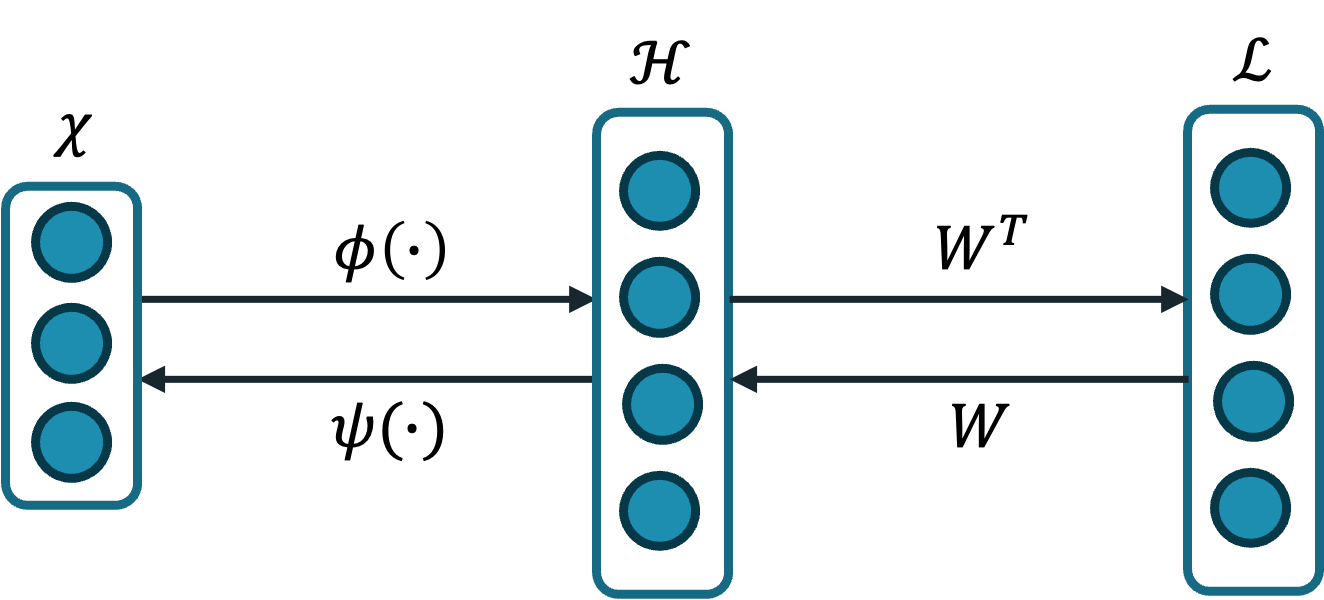
\includegraphics[width=0.7\linewidth]{Figures/PS/rkm_structure.png}
    \caption{Schematic representation of Gen-RKM. $\bphi(.)$ is the feature map network, while $\bpsi(.)$ corresponds to the pre-image network. $\bW$ is the interconnection matrix yielded from KPCA, mapping feature representations to the latent space $\mathcal{L}$. Latent points can be remapped back to the feature space via the transpose of the transformation matrix $\bW^{\top}$.}
    \label{rkm-demo}
\end{figure}

Next, a motivating example on the 012-MNIST dataset is used to illustrate the data imbalance issue in the Gen-RKM model. We consider an unbalanced version of the MNIST dataset, where only digits 0-2 are included and digit 2 is set to the minority class (see Section \ref{subsec-expr-datasets} for a more detailed introduction about the dataset used). Figure \ref{fig-latent-ub} (first row) shows the yielded latent space on the 012-MNIST dataset and the unbalanced version of it in the Gen-RKM setting. In the balanced dataset, well-separated or distinguishable clusters are produced in the latent space, and the corresponding latent representations are (nearly) evenly distributed, indicating each class has a similar influence on the learned latent space. As for the unbalanced scenario, it can be clearly observed that the learned latent space is strongly biased toward the majority groups since latent points from minority modes are mostly blurred or intermixed with the majority modes. The impact of data imbalance is significant on the latent space representation, where minority modes (or classes) are underrepresented, potentially leading to challenges in the generation or reconstruction of the underrepresented groups.

Data imbalance also has a similar effect on VAE as showcased in Figure \ref{fig-latent-ub} (second row), where the minority classes tend to be biased by the majority classes. That is unsurprising, as Gen-RKM and VAE share similar encoder-decoder architectures, and the data distribution in both models is explicitly defined. The biases in the final generation results brought by data imbalance are confirmed in Figure \ref{fig-mnist}, where random generations from both balanced and unbalanced datasets are depicted. One can observe that samples from minority classes are generated much less frequently than those from majority classes.

To extend the capability of Gen-RKM to generalize well to the minority classes in the unbalanced data, a natural idea is to augment the minority classes in the latent space (in other words, synthetically increasing the number of latent points corresponding to minority modes). In this spirit, the generation result should be more diverse. Of course, this approach is equivalent to performing augmentation on the original data, as only a balanced distribution of raw data can result in a balanced distribution in its corresponding latent space. In the next chapter, we will discuss random sampling, a naive yet effective approach for addressing data imbalance. Specifically, we will combine various sampling techniques with Gen-RKM  framework to investigate how to tackle the issue of unbalanced data in the generative learning context.

% Figure \ref{fig-latent-ub} shows the latent space of the MNIST012 datasets and the unbalanced version of it. When the dataset is unbalanced (The number of digit 2 is only 10\% of the numbers of 0 and 1), it is hard to observe the representation of the minority class in the latent space. And GMM estimation tends to treat these minorities as noise, resulting in a low probability of sampling from these groups when generating new samples. Figure \ref{fig-mnist} compares the randomly generated samples from the latent spaces in Figure \ref{fig-latent-ub} respectively. There are almost no samples from minority classes generated from the unbalanced latent space. 




\begin{figure}[H]
    \centering
    \begin{subfigure}{0.45\textwidth}
        \centering
        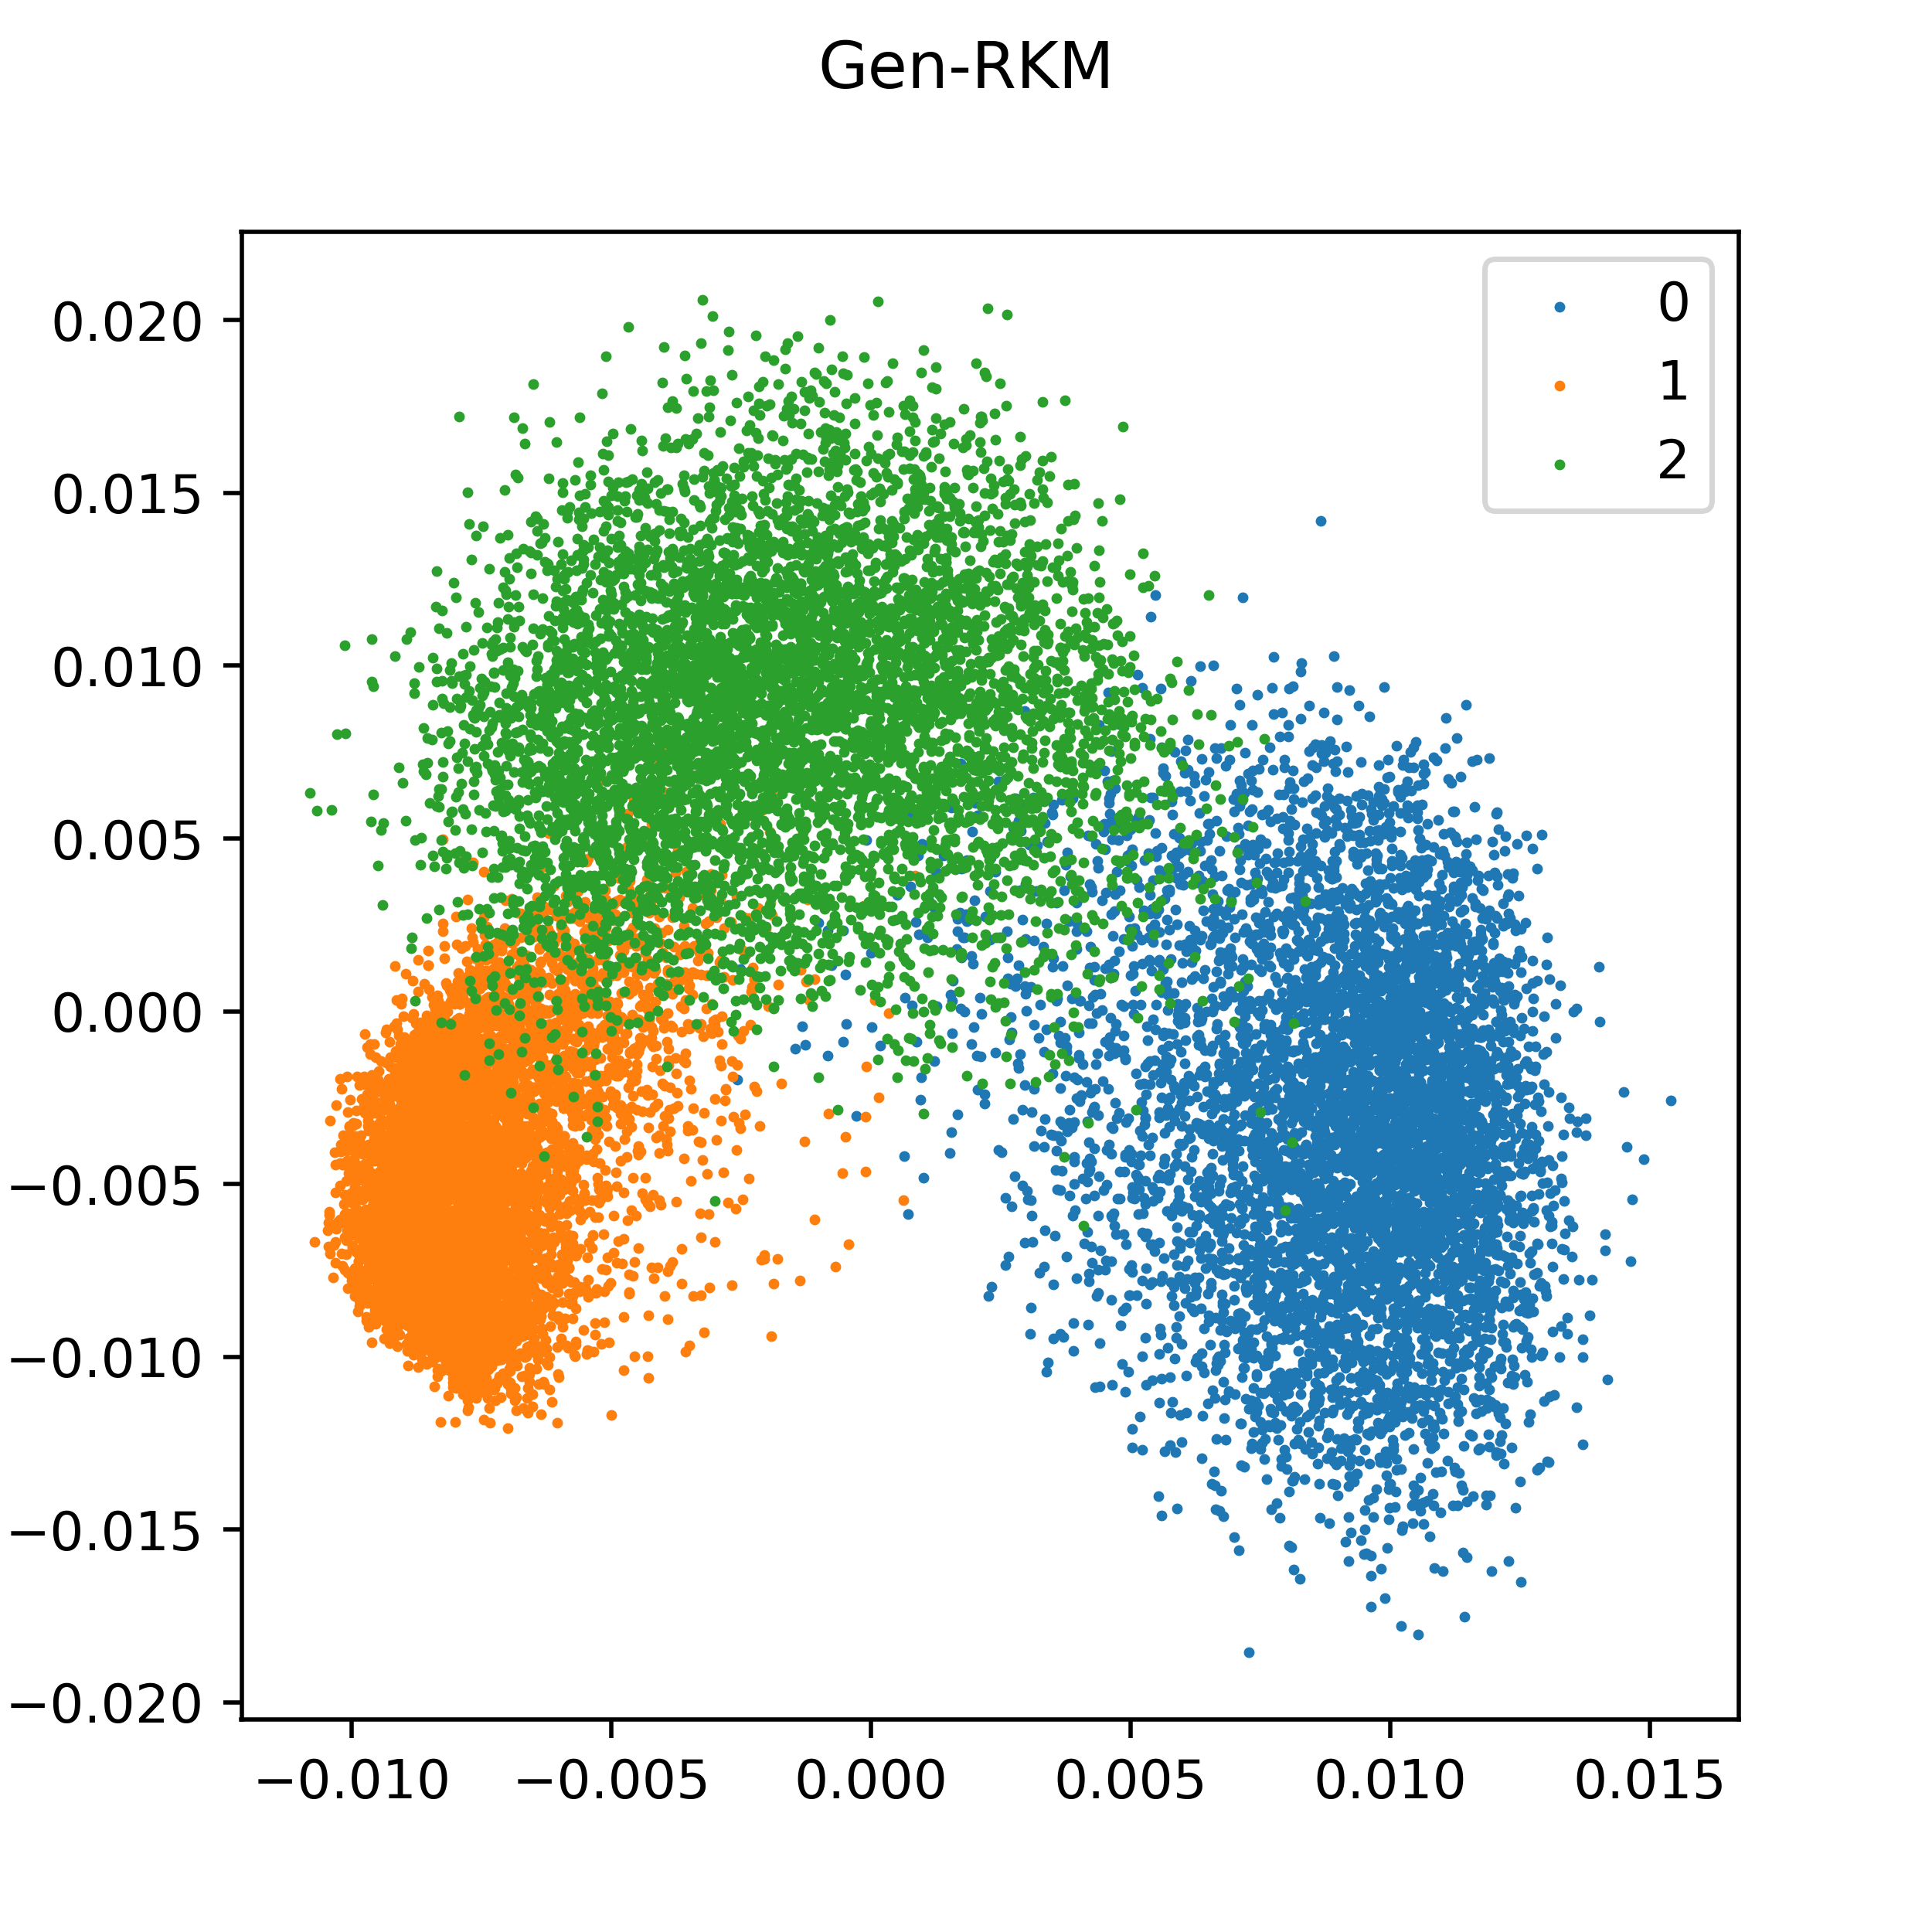
\includegraphics[width=0.8\textwidth]{Figures/PS_v2/rkm-bMNIST012-latentspace-vis.png}
    \end{subfigure}
    \hfill
    \begin{subfigure}{0.45\textwidth}
        \centering
        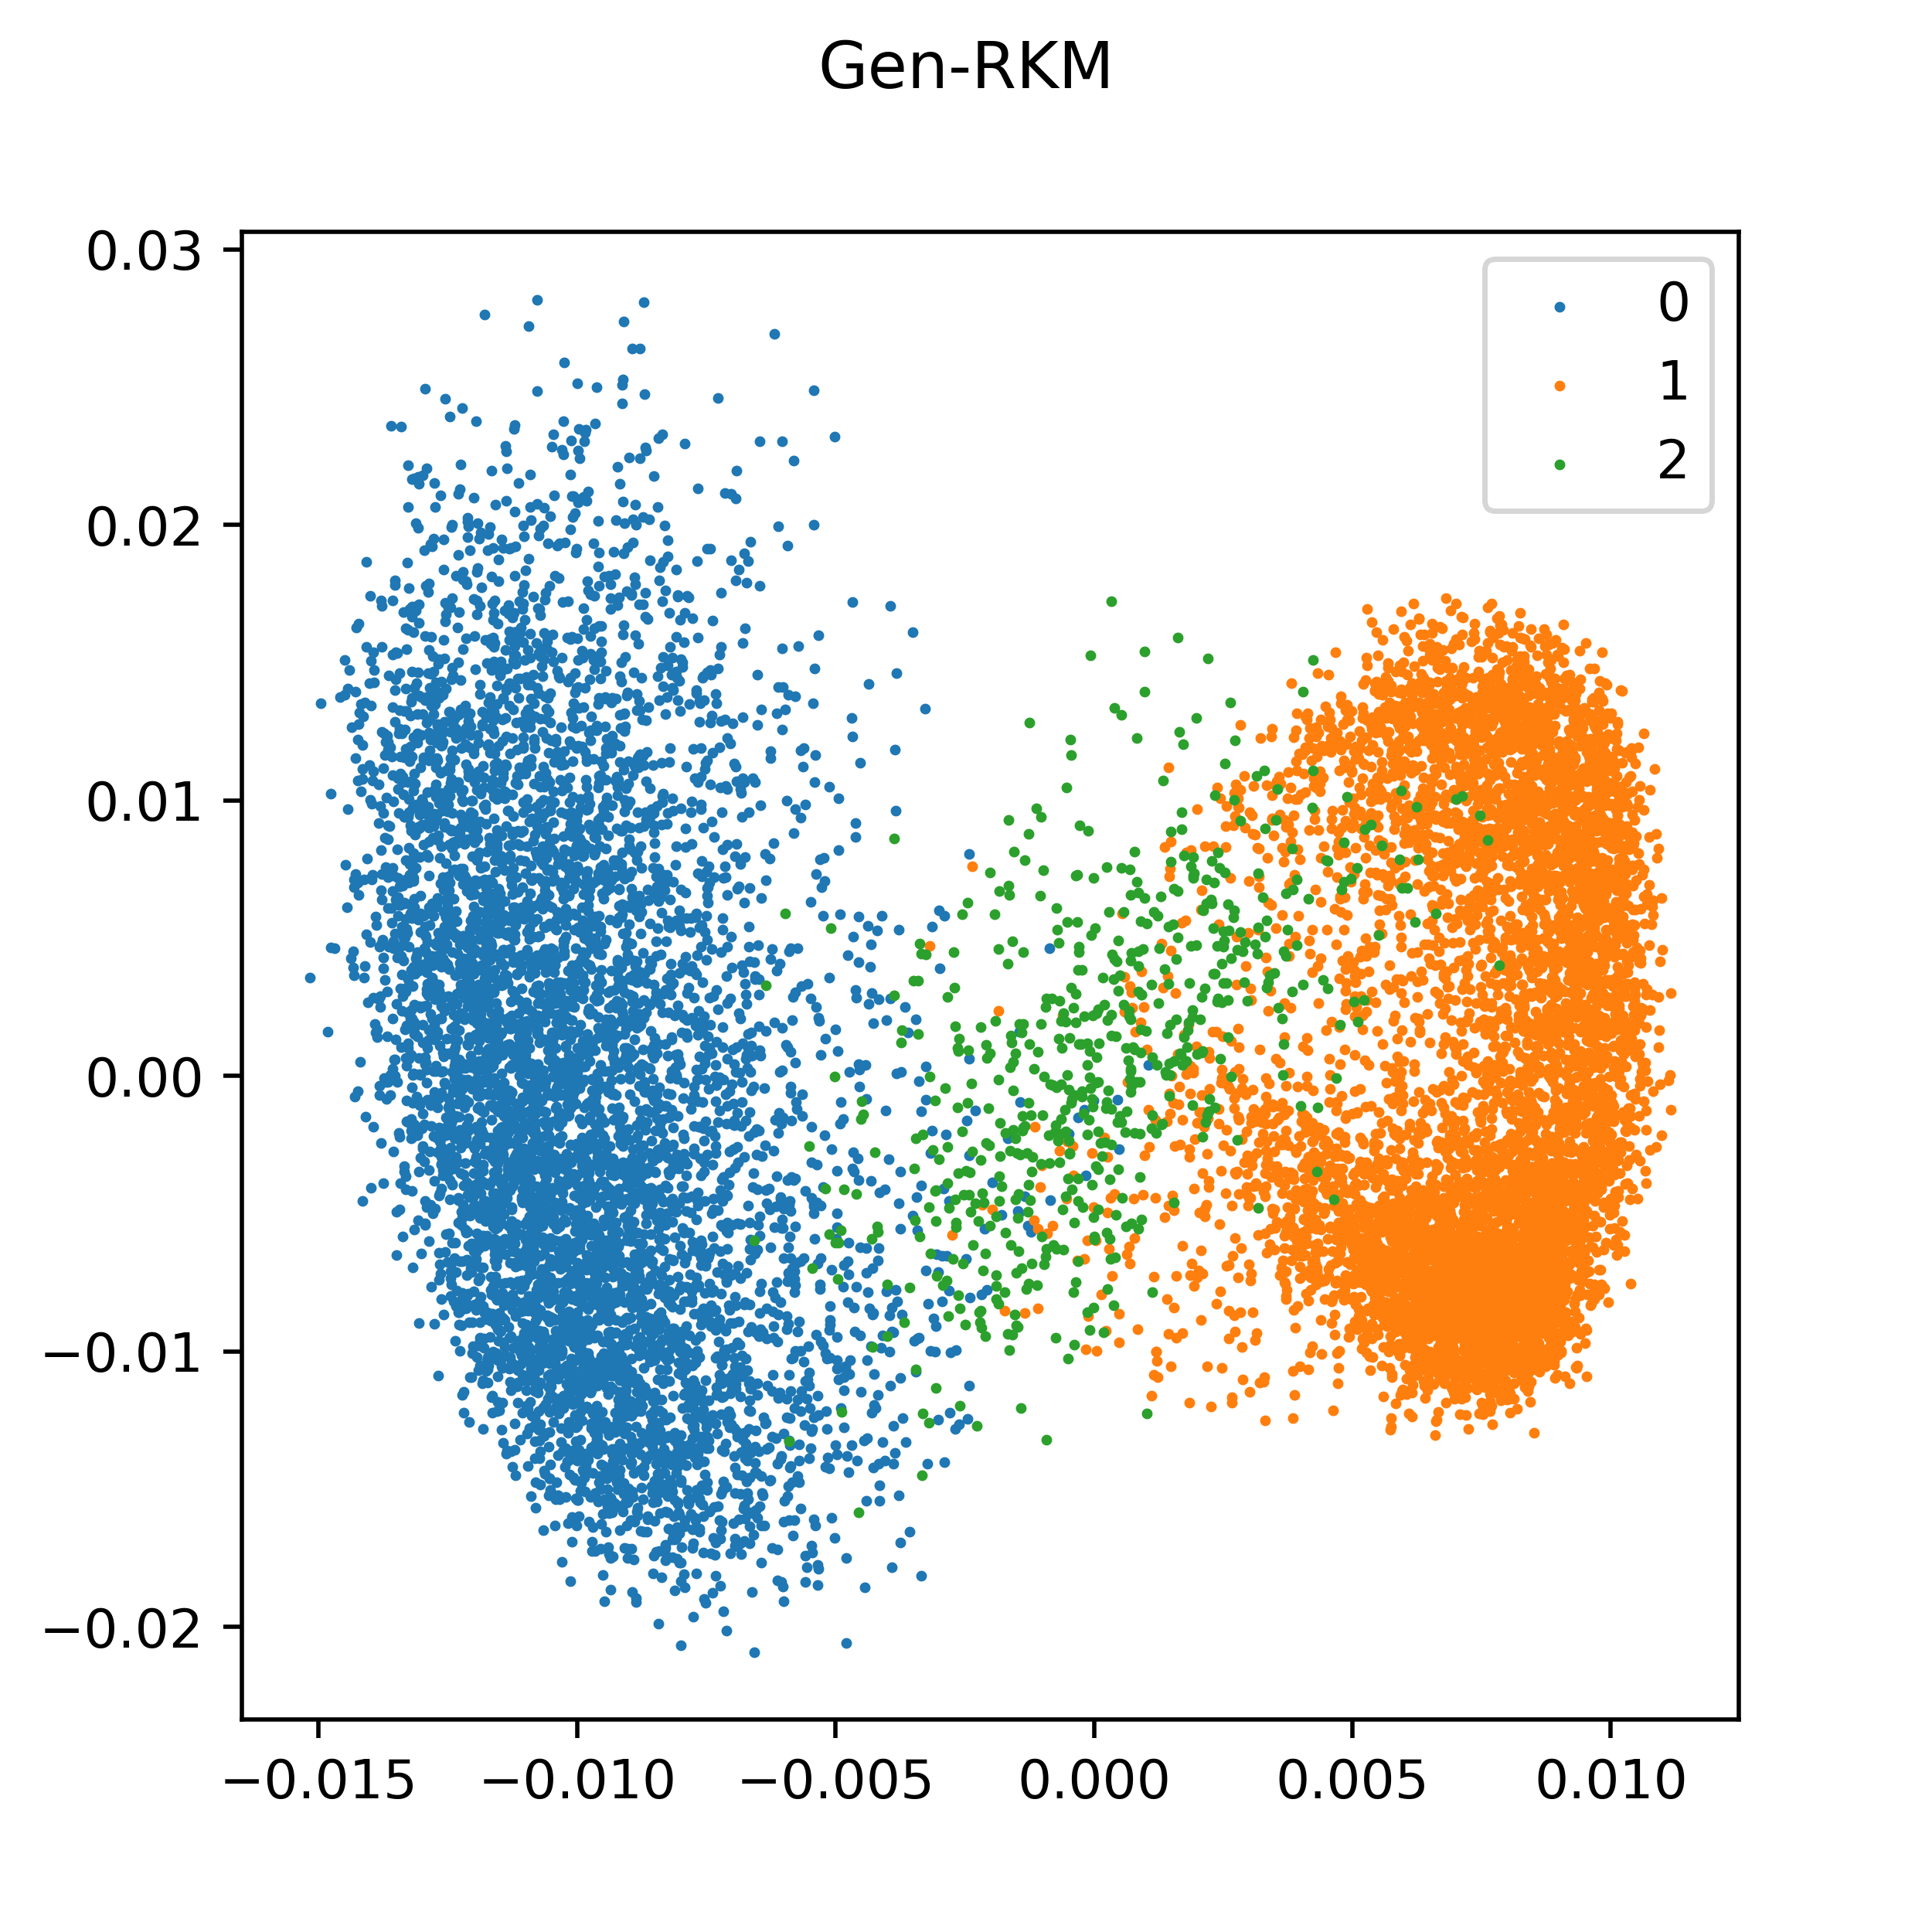
\includegraphics[width=0.8\textwidth]{Figures/PS_v2/rkm-ubMNIST012-latentspace-vis.png}
    \end{subfigure}
    \vfill
    \begin{subfigure}{0.45\textwidth}
        \centering
        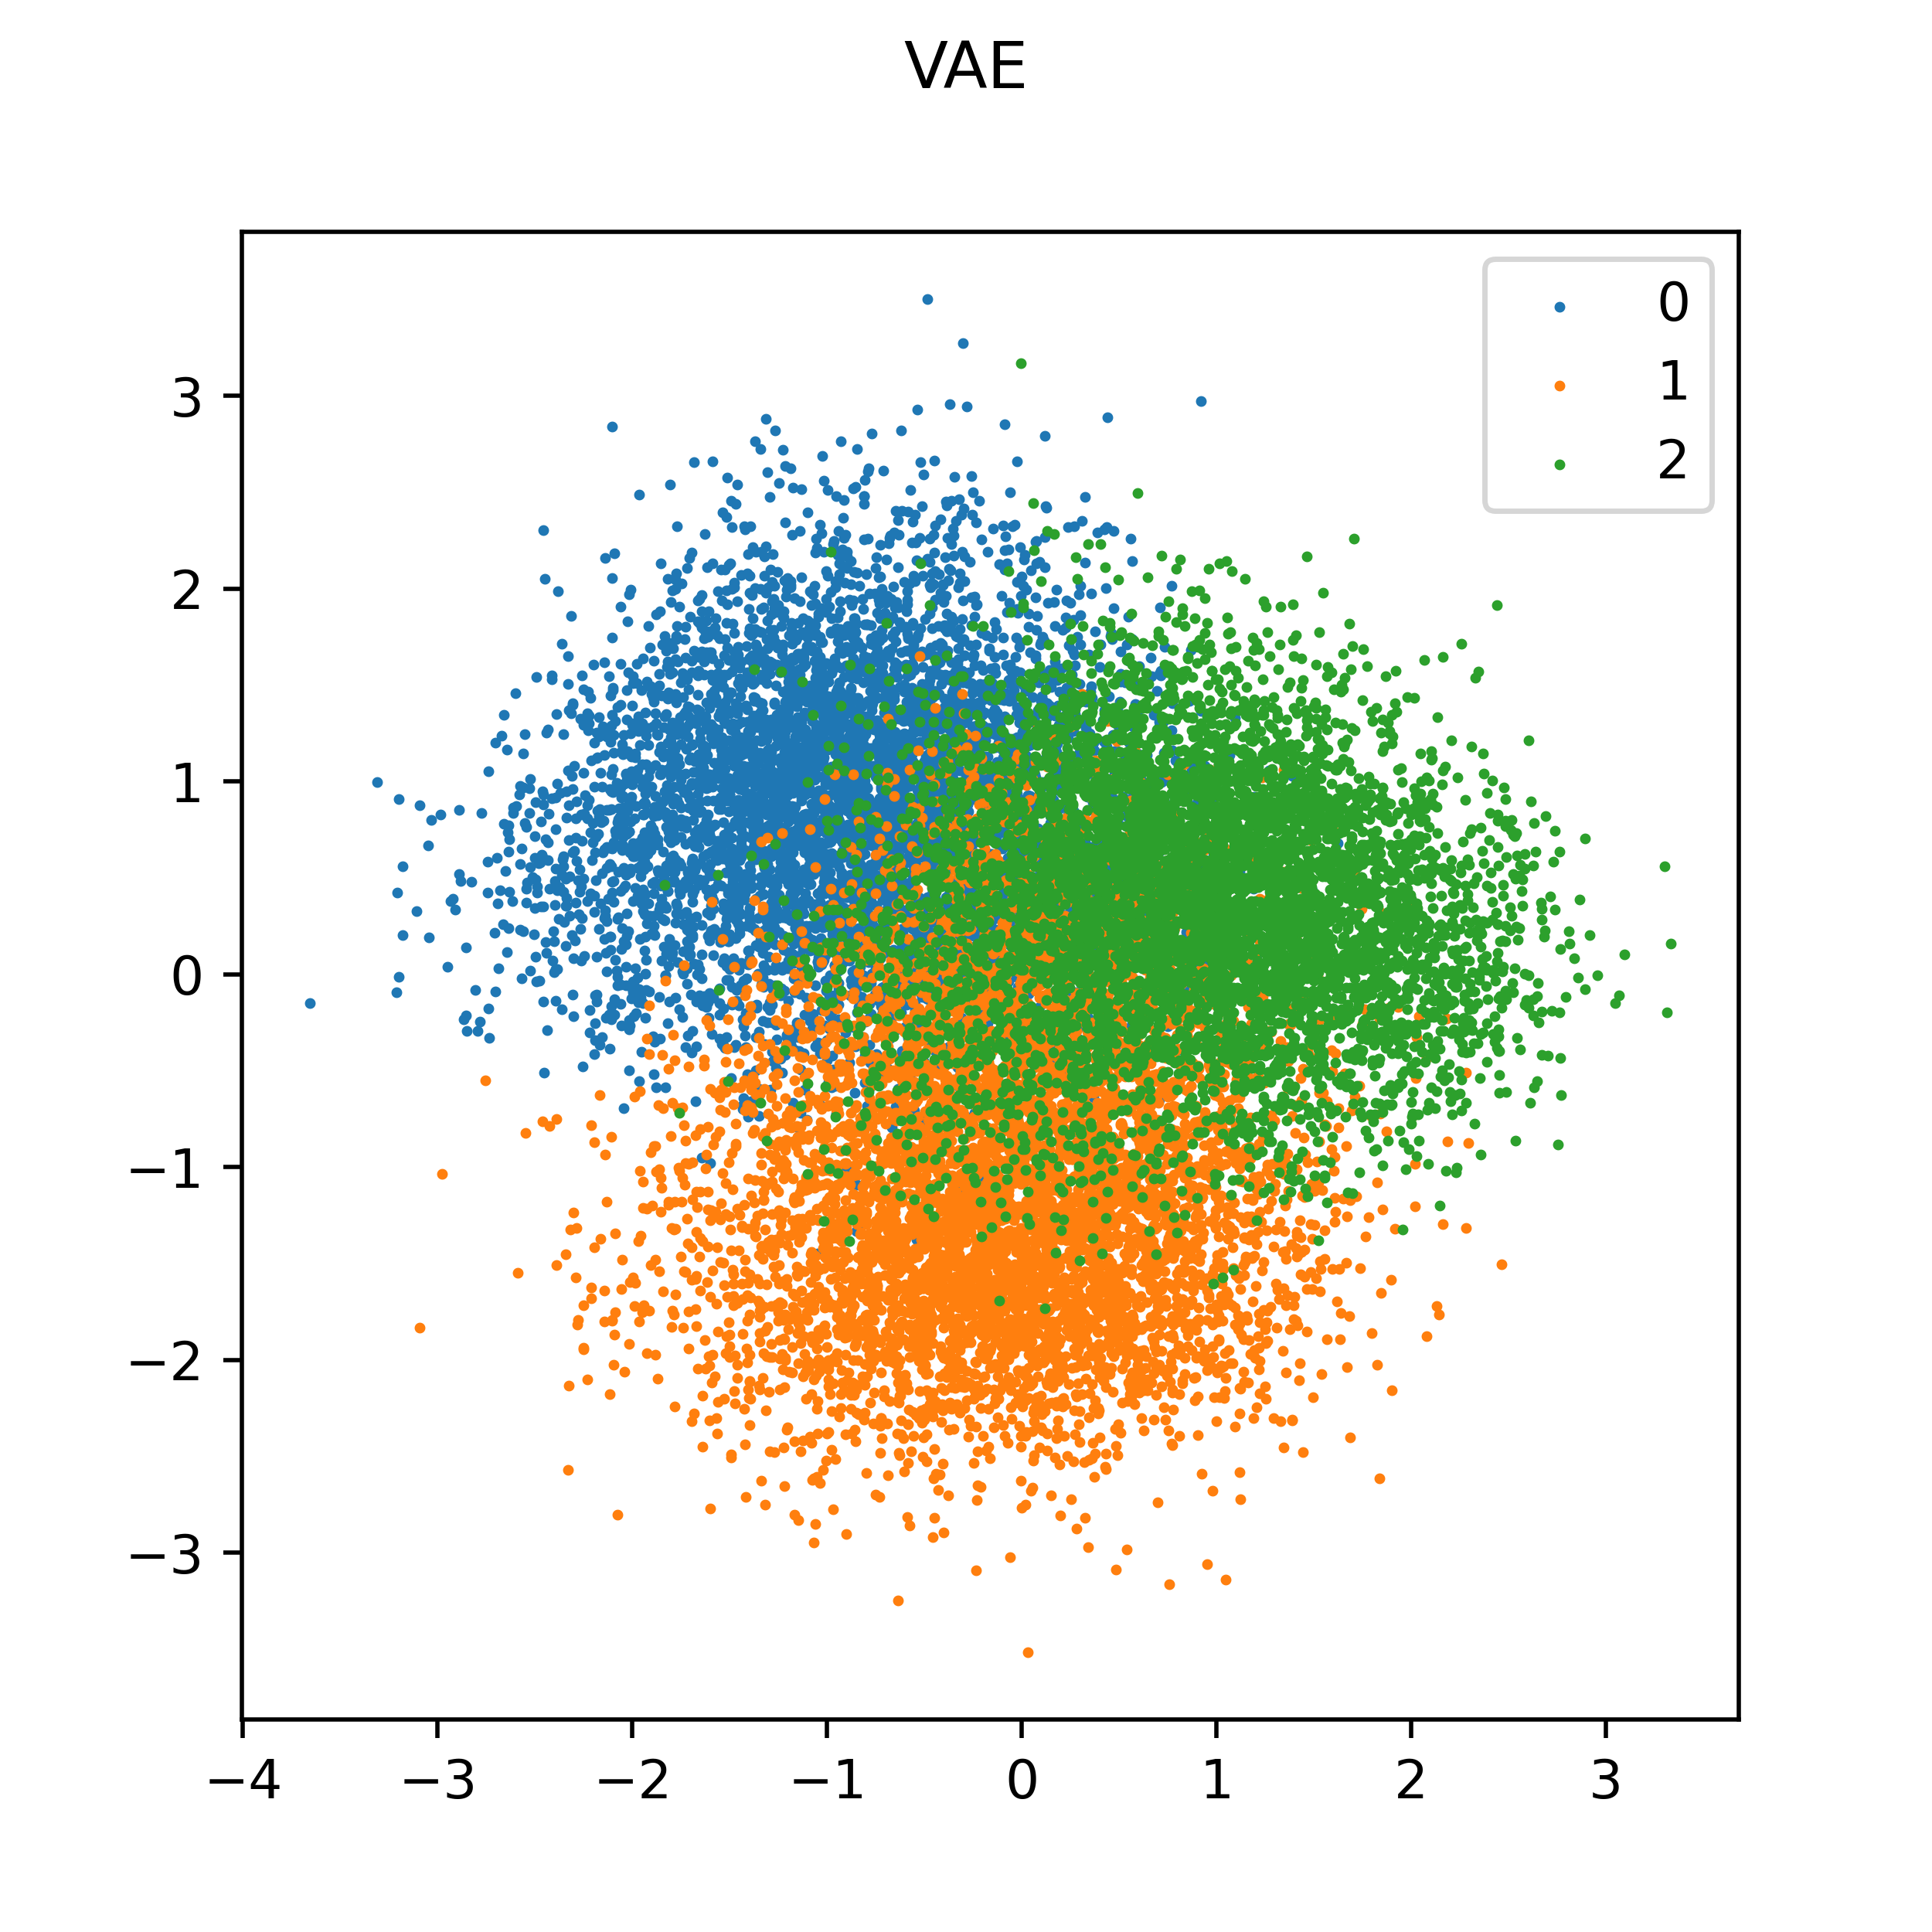
\includegraphics[width=0.8\textwidth]{Figures/PS_v2/vae-bMNIST012-latentspace-vis.png} % Replace with your third image path
    \end{subfigure}
    \hfill
    \begin{subfigure}{0.45\textwidth}
        \centering
        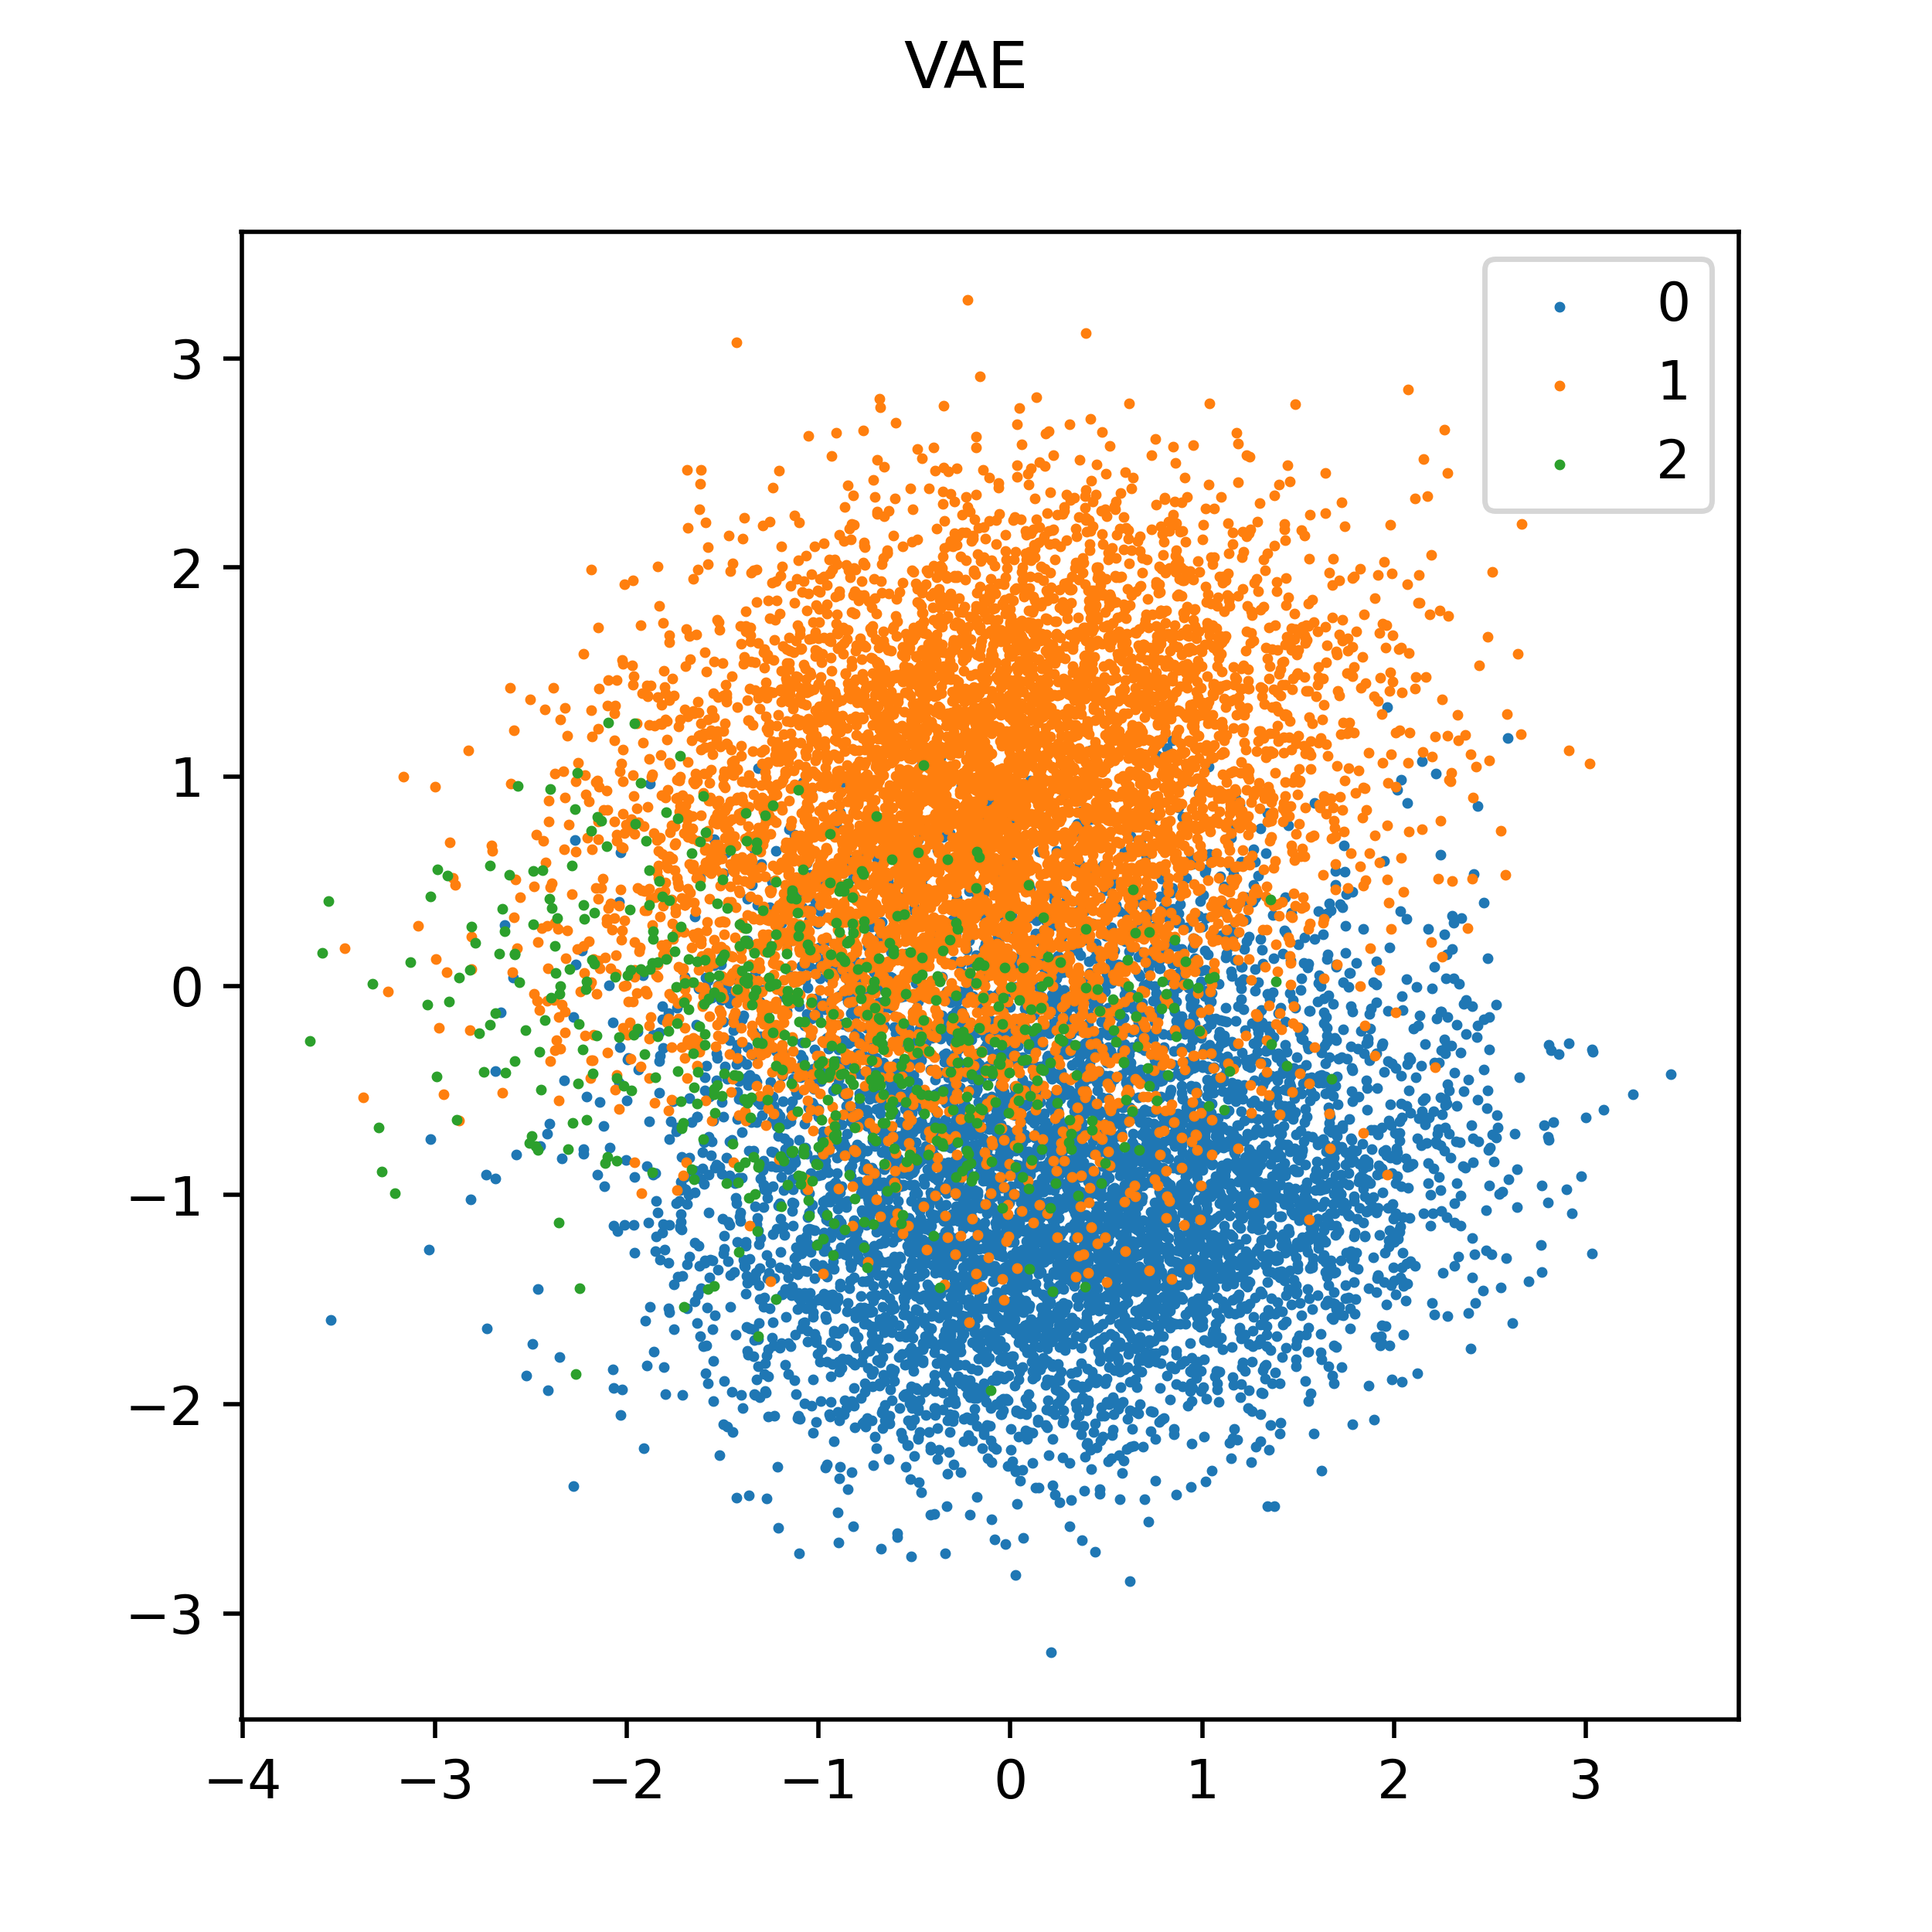
\includegraphics[width=0.8\textwidth]{Figures/PS_v2/vae-ubMNIST012-latentspace-vis.png} % Replace with your fourth image path
    \end{subfigure}
    \caption{Visualizations of latent spaces of Gen-RKM (first row) and VAE (second row) trained on balanced (first column) and unbalanced 012-MNIST datasets (second columns). The minority mode is depicted in green color. Sizes of latent space of both Gen-RKM and VAE are set to 10, and only the first two dimensions are visualized.}
    \label{fig-latent-ub}
\end{figure}


% \begin{figure}[H]
%     \centering
%     \begin{subfigure}{0.45\textwidth}
%         \centering
%         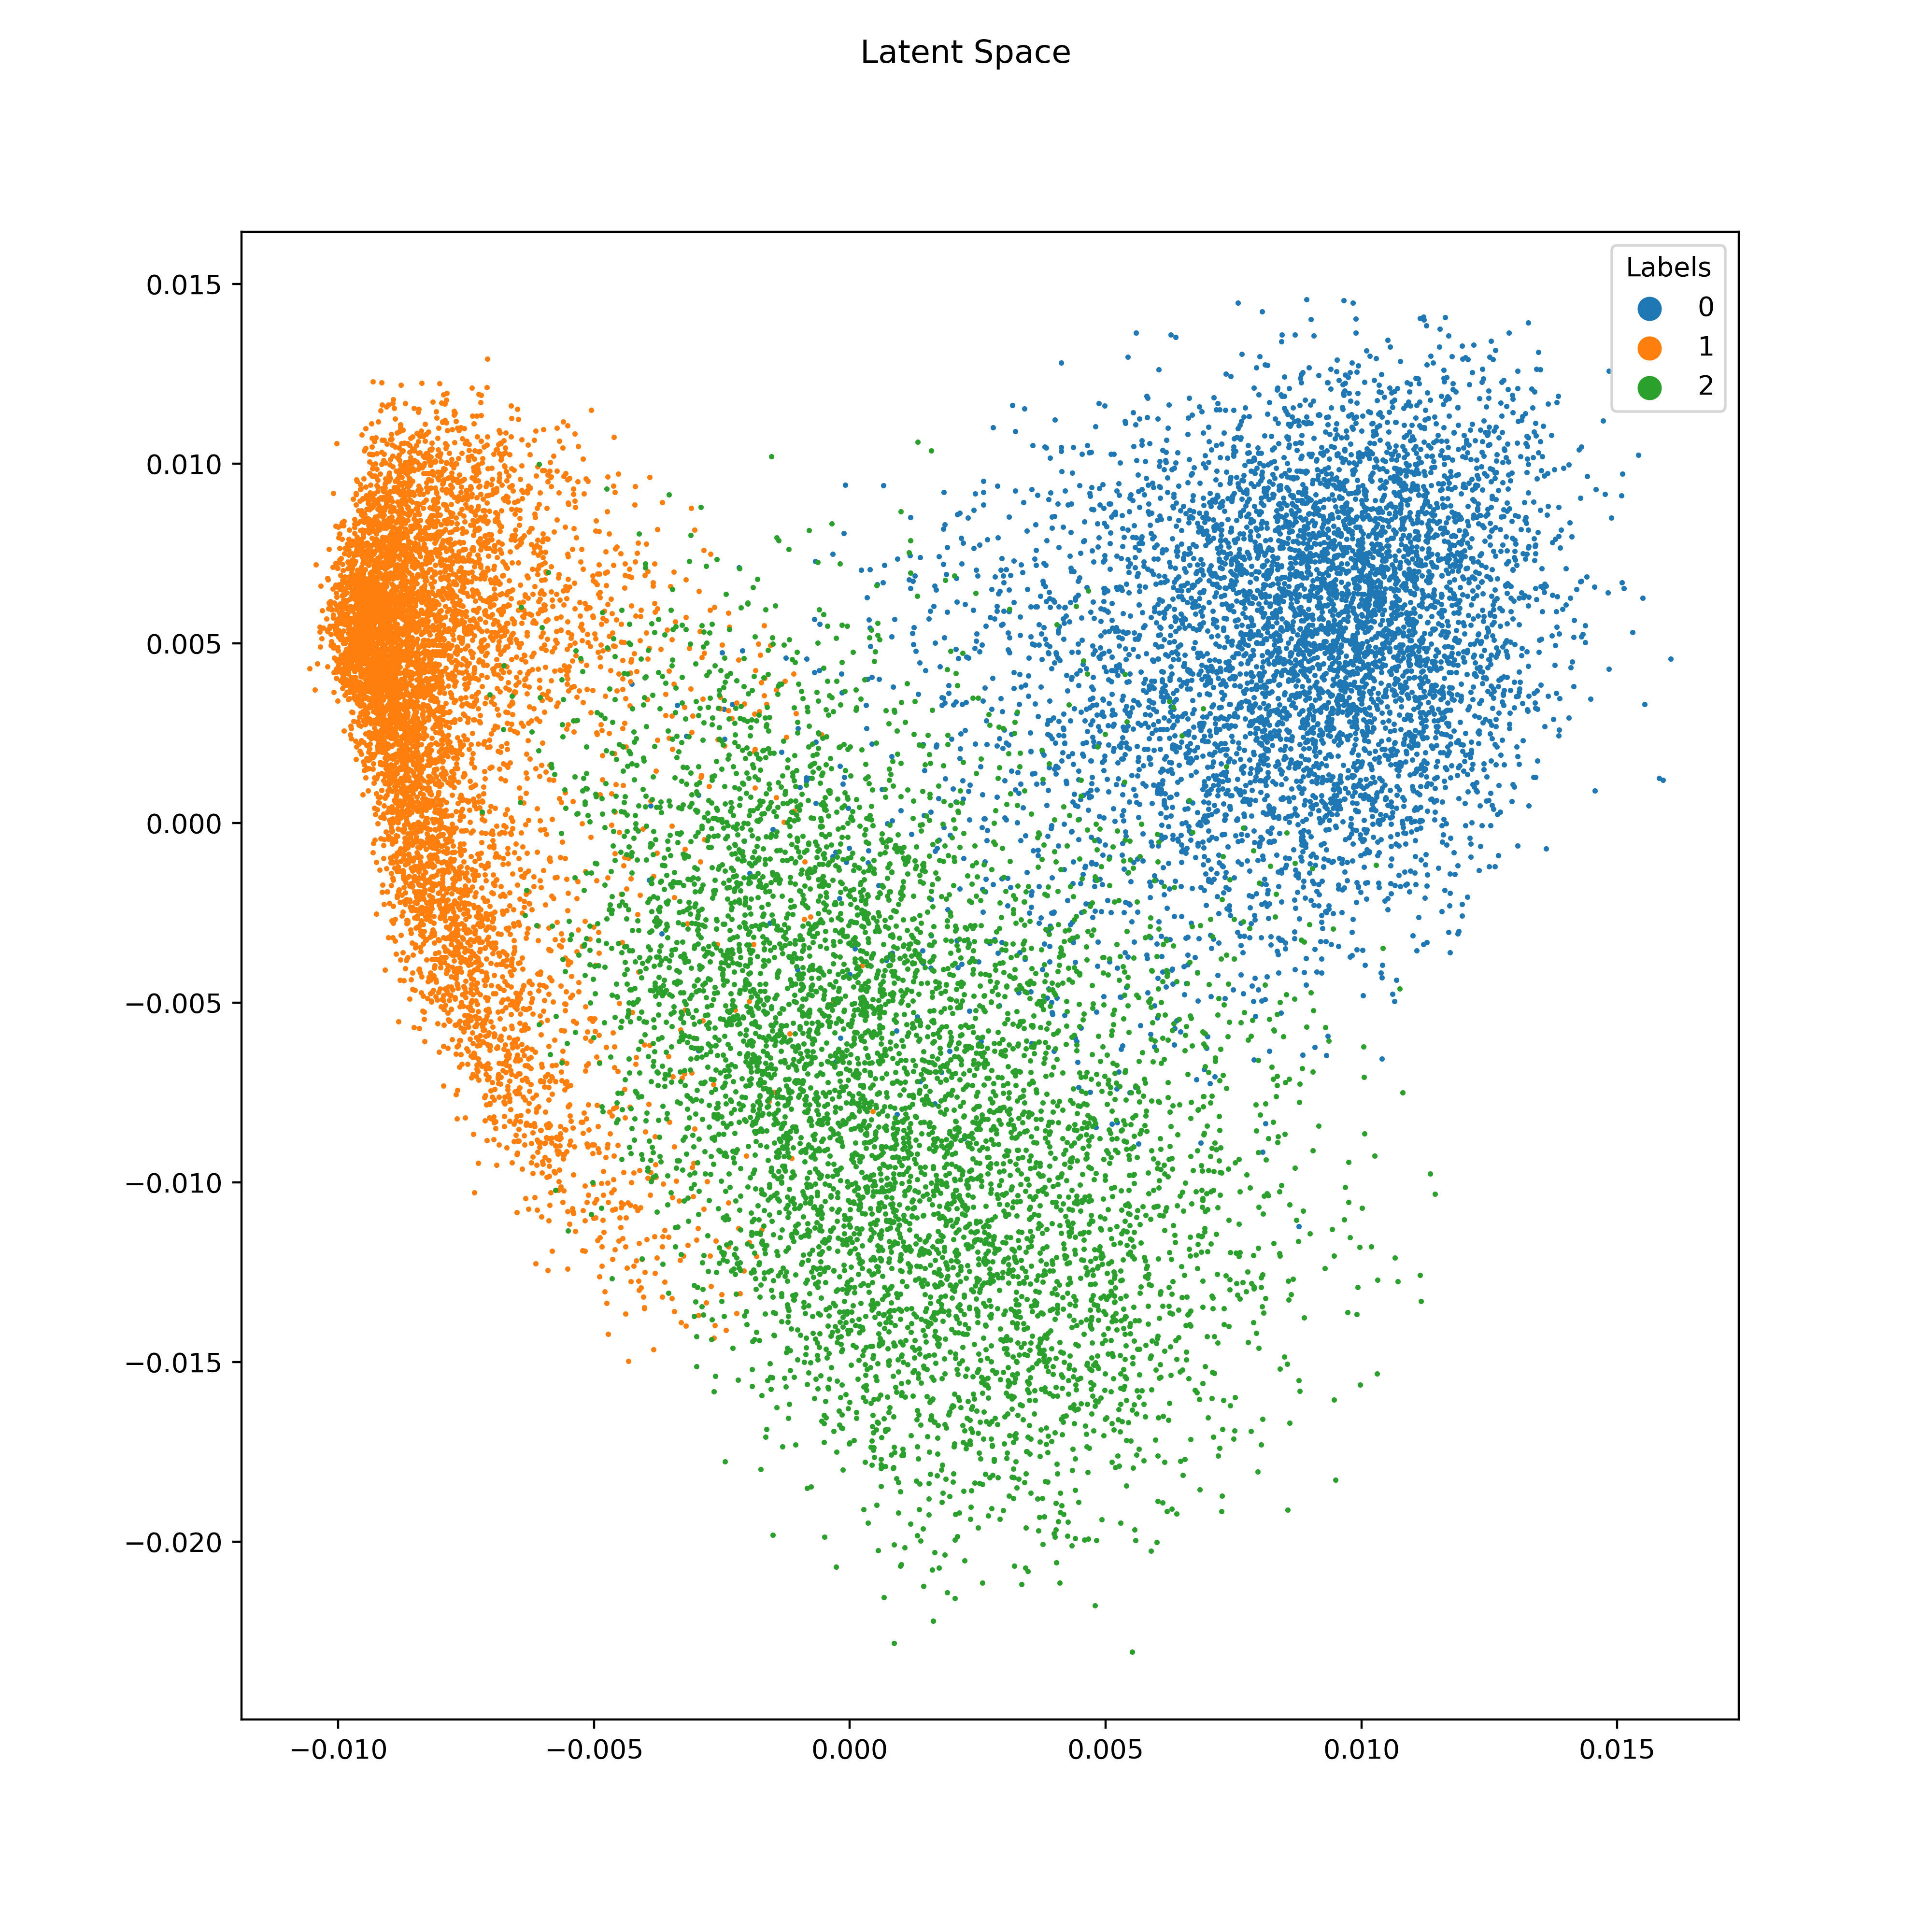
\includegraphics[width=0.8\textwidth]{Figures/PS/b012_latent_space.png}
%     \end{subfigure}
%     \hfill
%     \begin{subfigure}{0.45\textwidth}
%         \centering
%         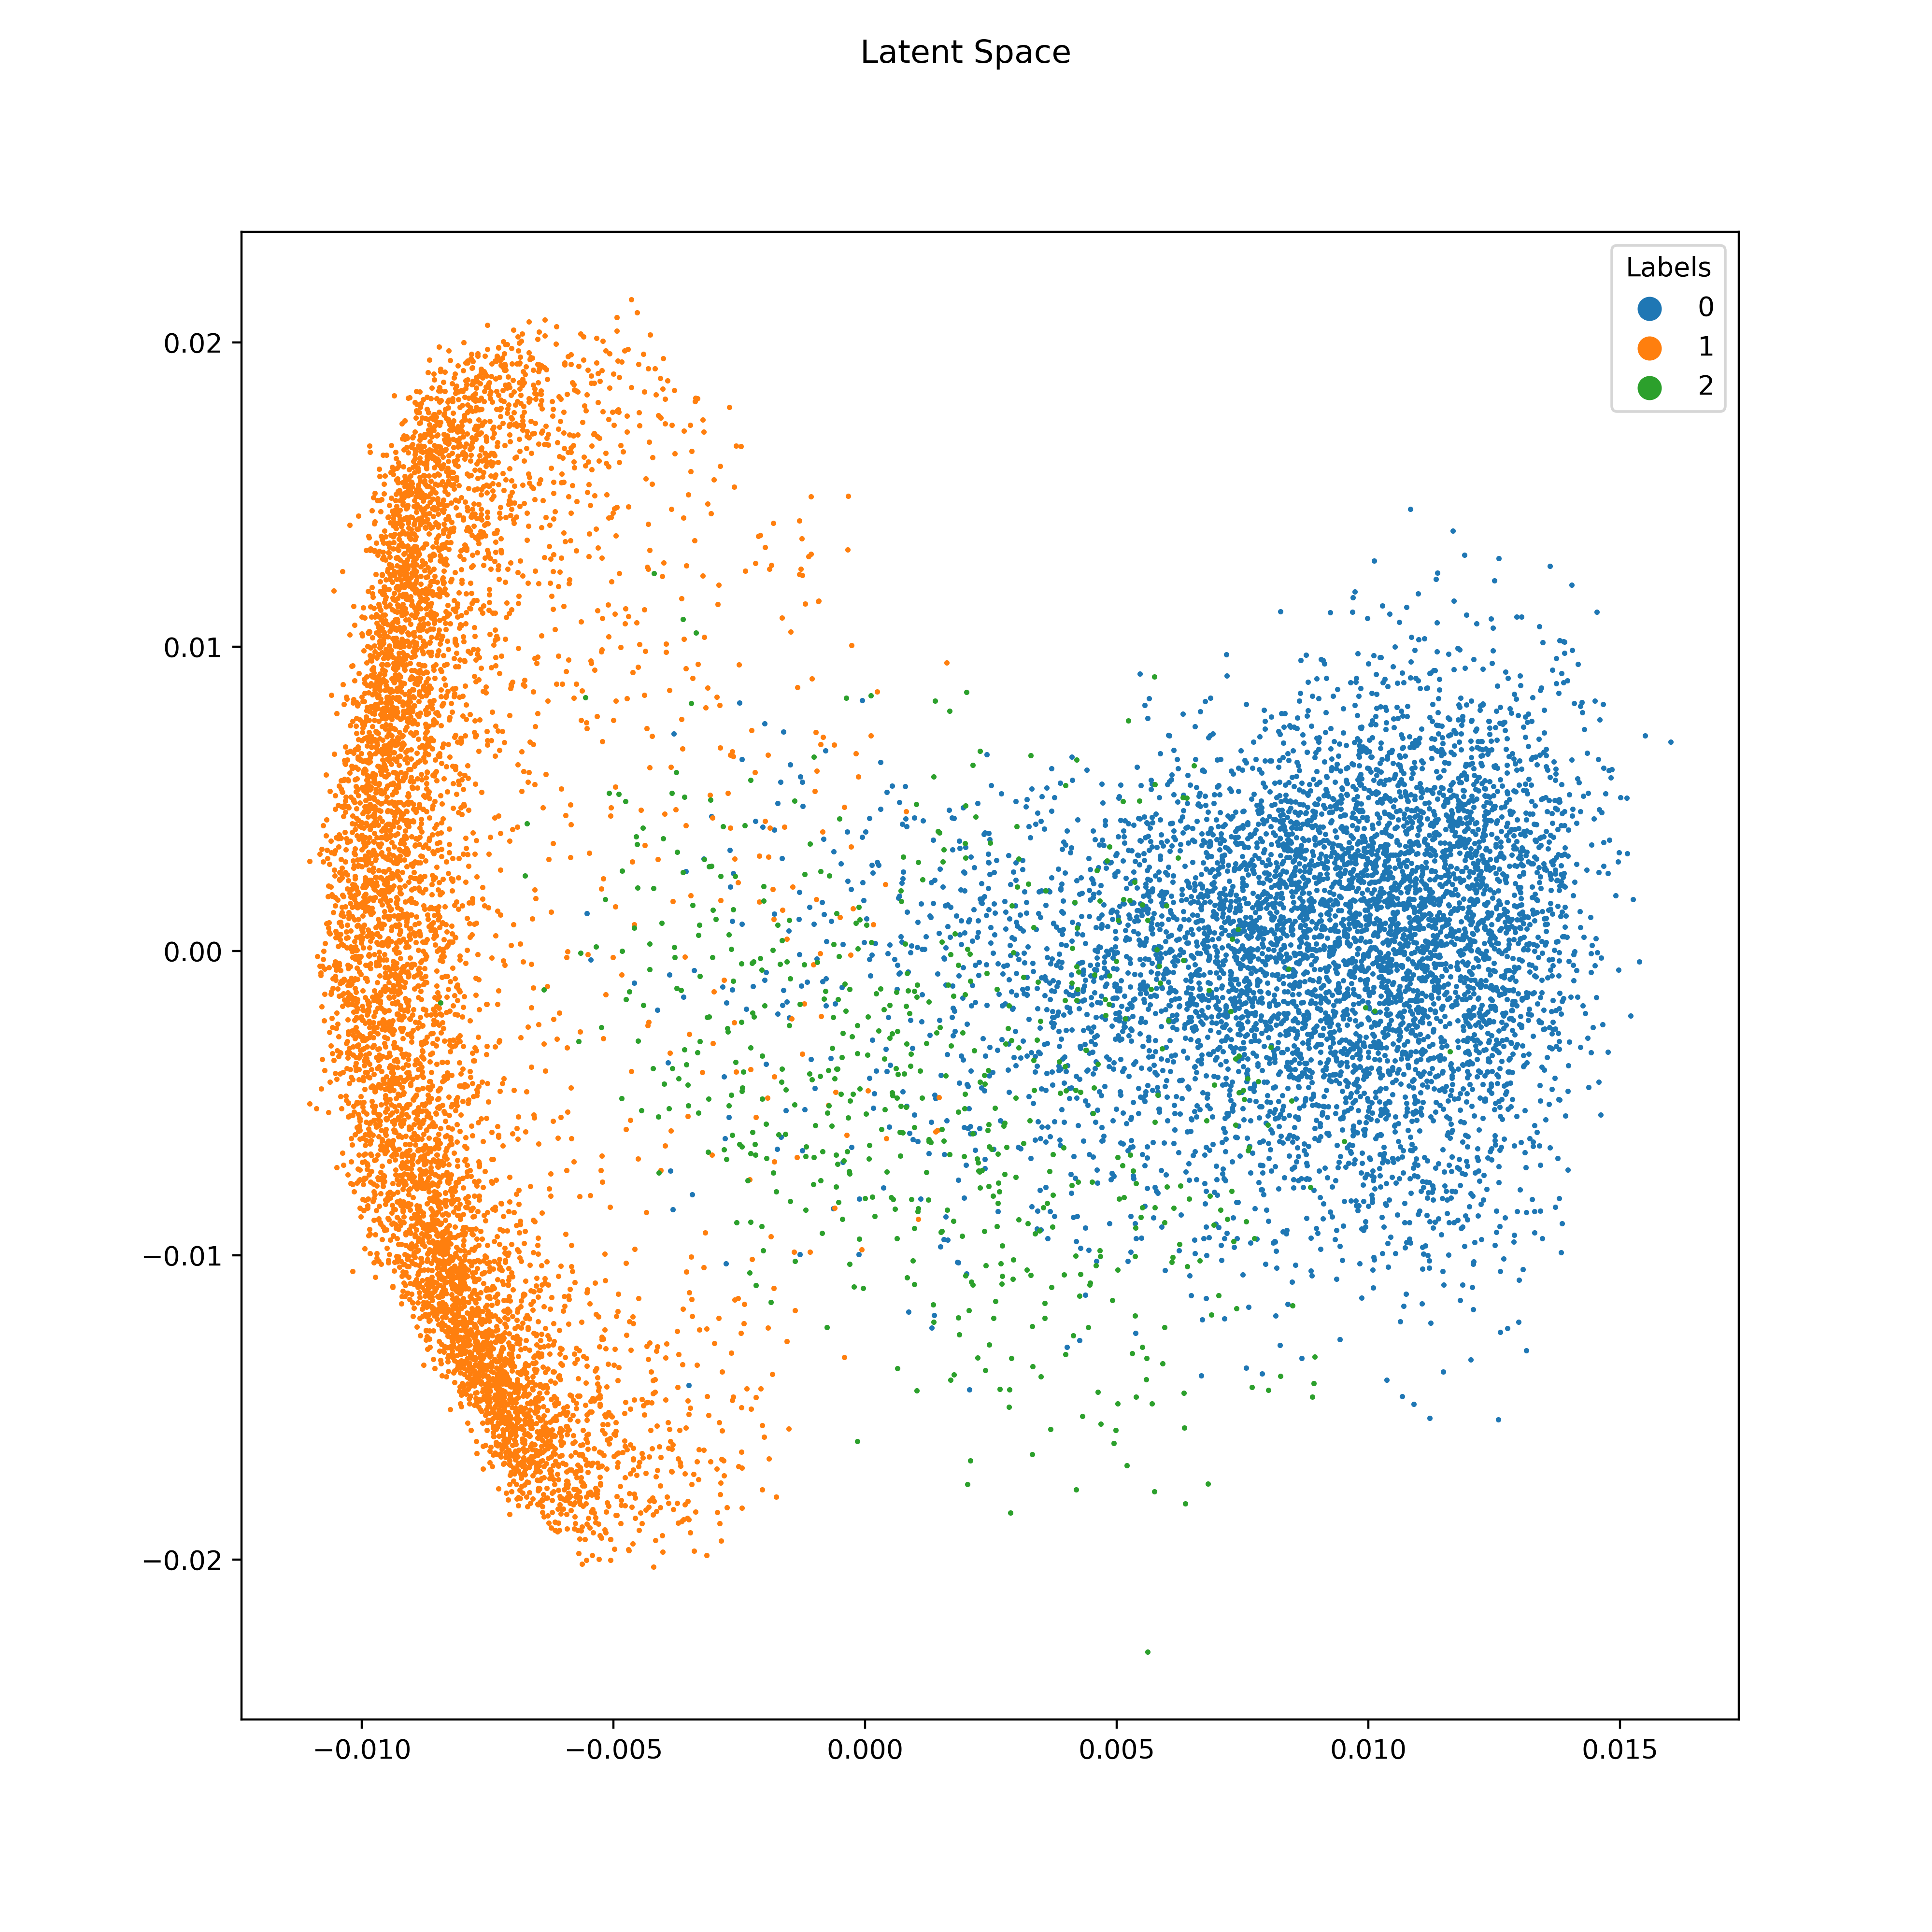
\includegraphics[width=0.8\textwidth]{Figures/PS/ub012_latent_space.png}
%     \end{subfigure}
%     \caption{Latent space of 012-MNIST: balanced (left) and unbalanced(right)}
%     \label{fig-latent-ub}
% \end{figure}

% \begin{figure}[H]
%     \centering
%     \begin{subfigure}{0.45\textwidth}
%         \centering
%         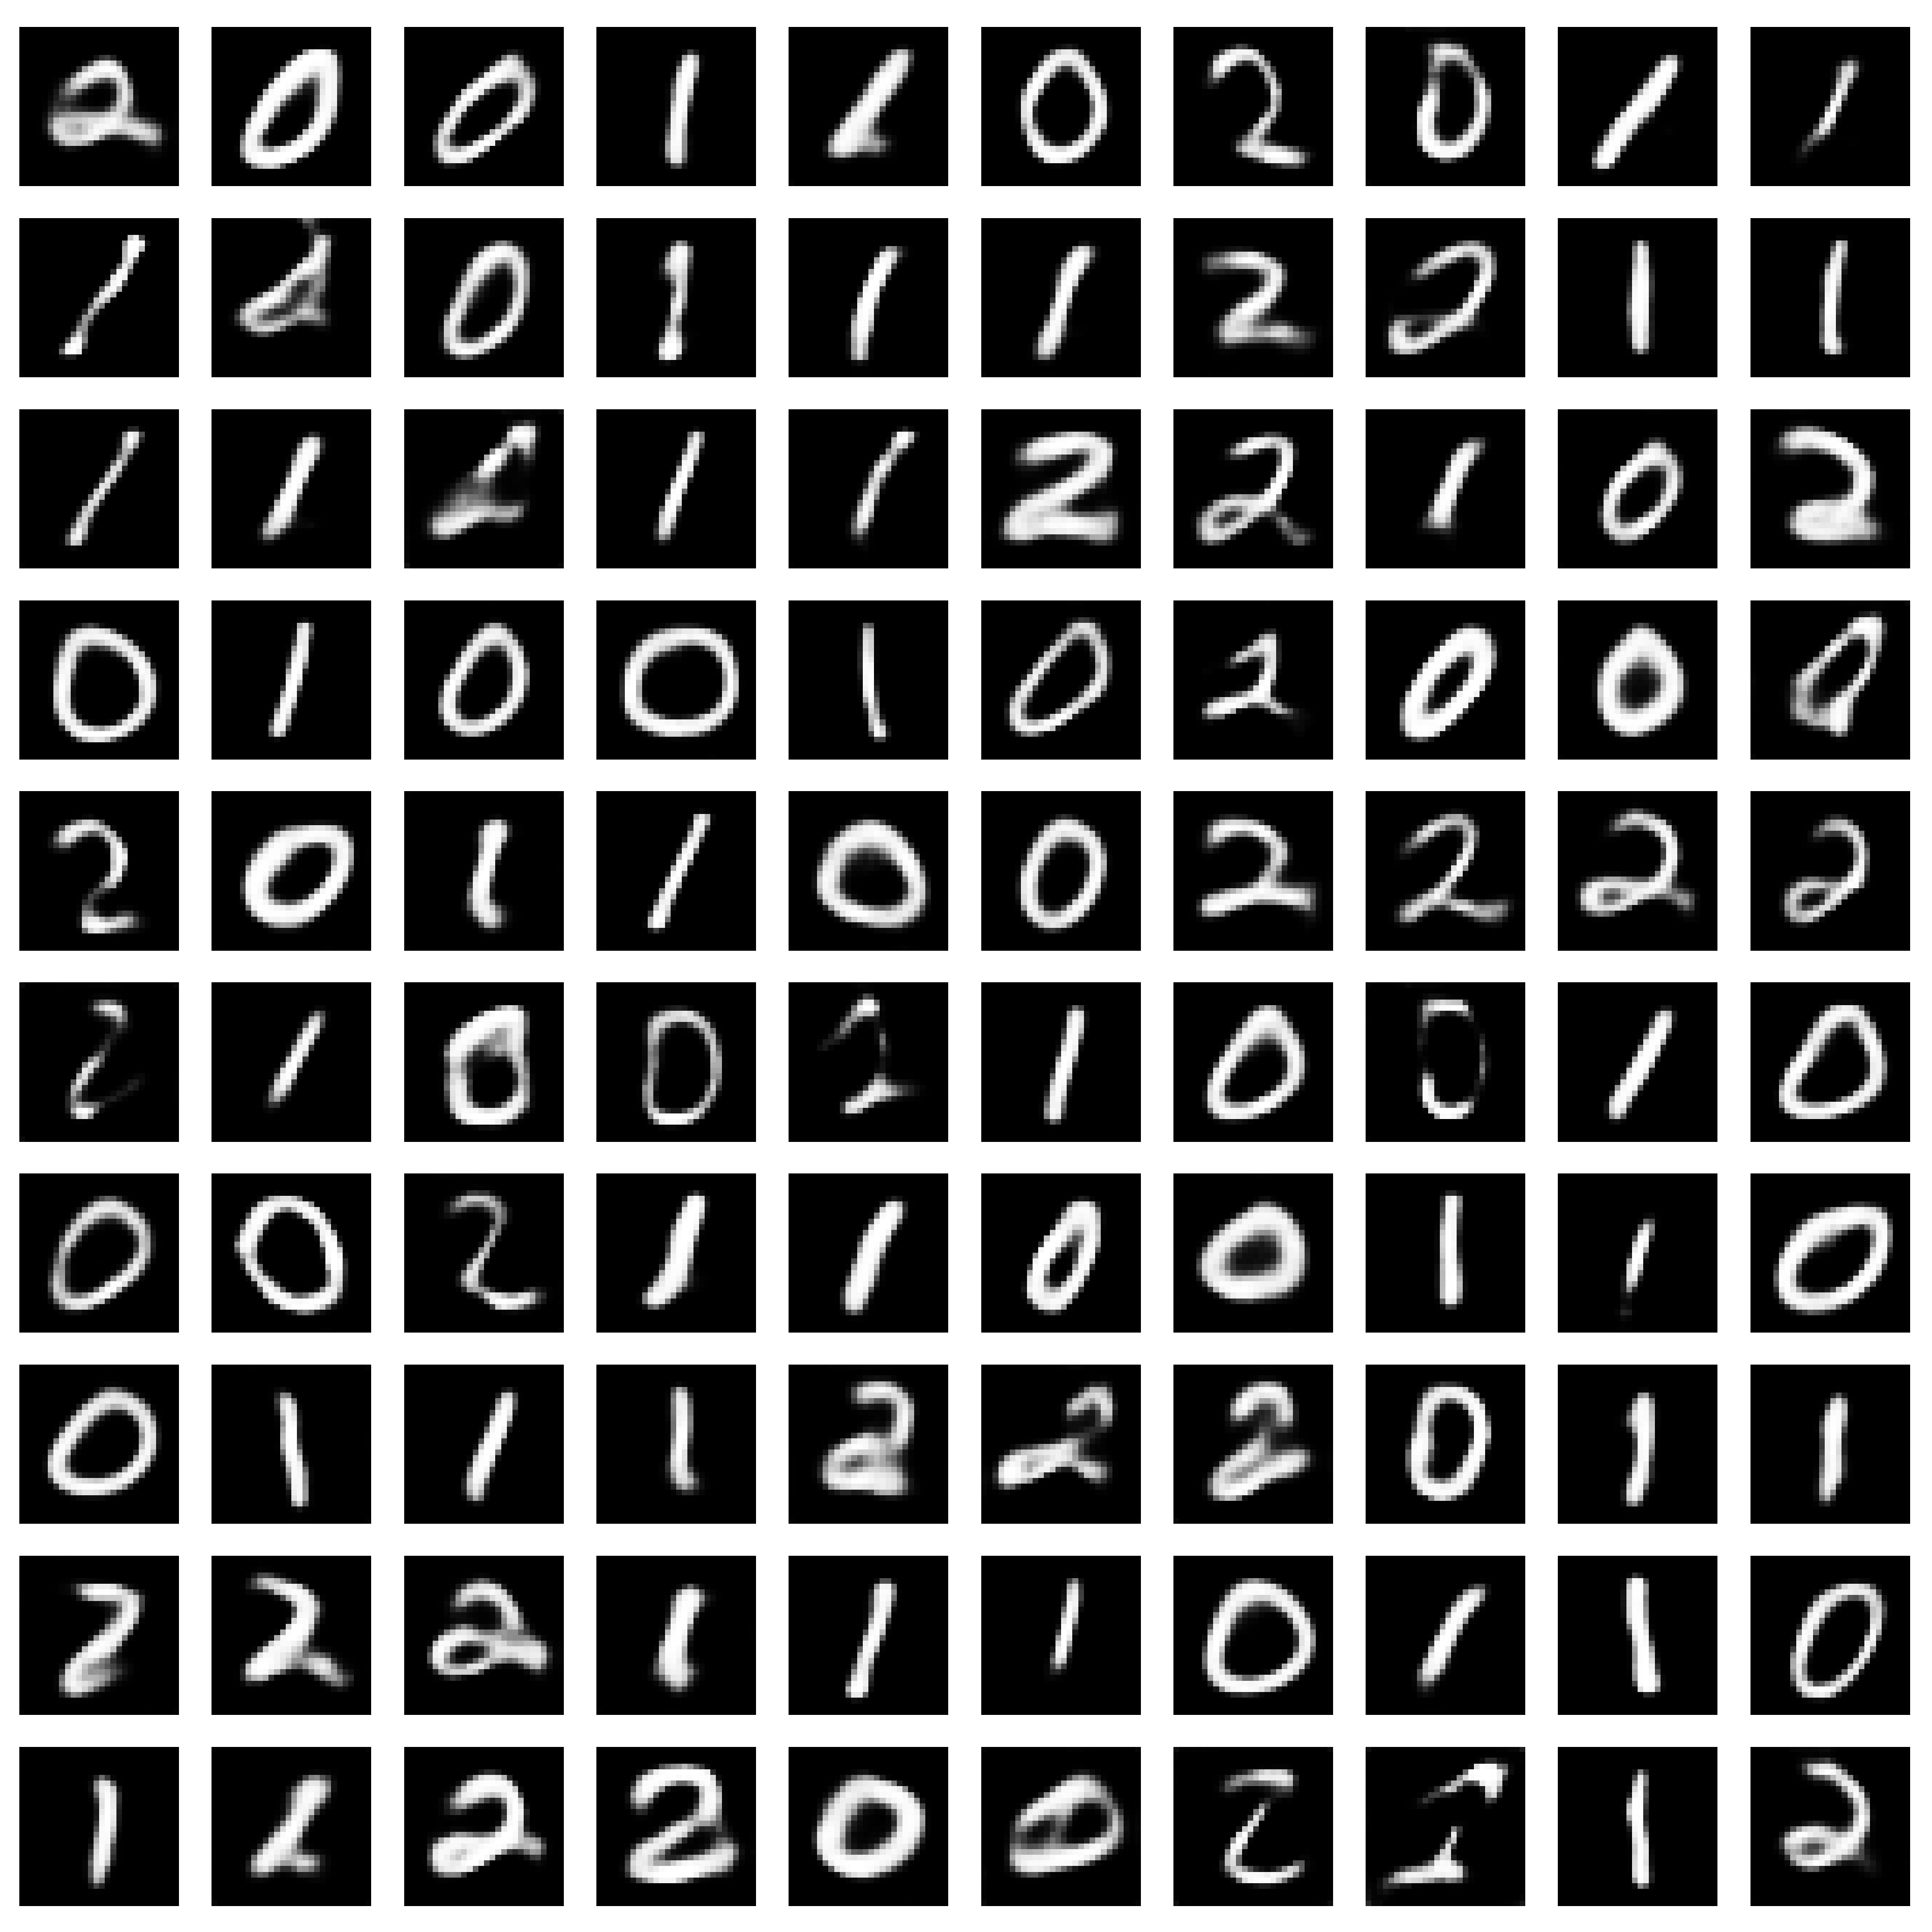
\includegraphics[width=0.8\textwidth]{Figures/PS/b012_random_generation.png}
%     \end{subfigure}
%     \hfill
%     \begin{subfigure}{0.45\textwidth}
%         \centering
%         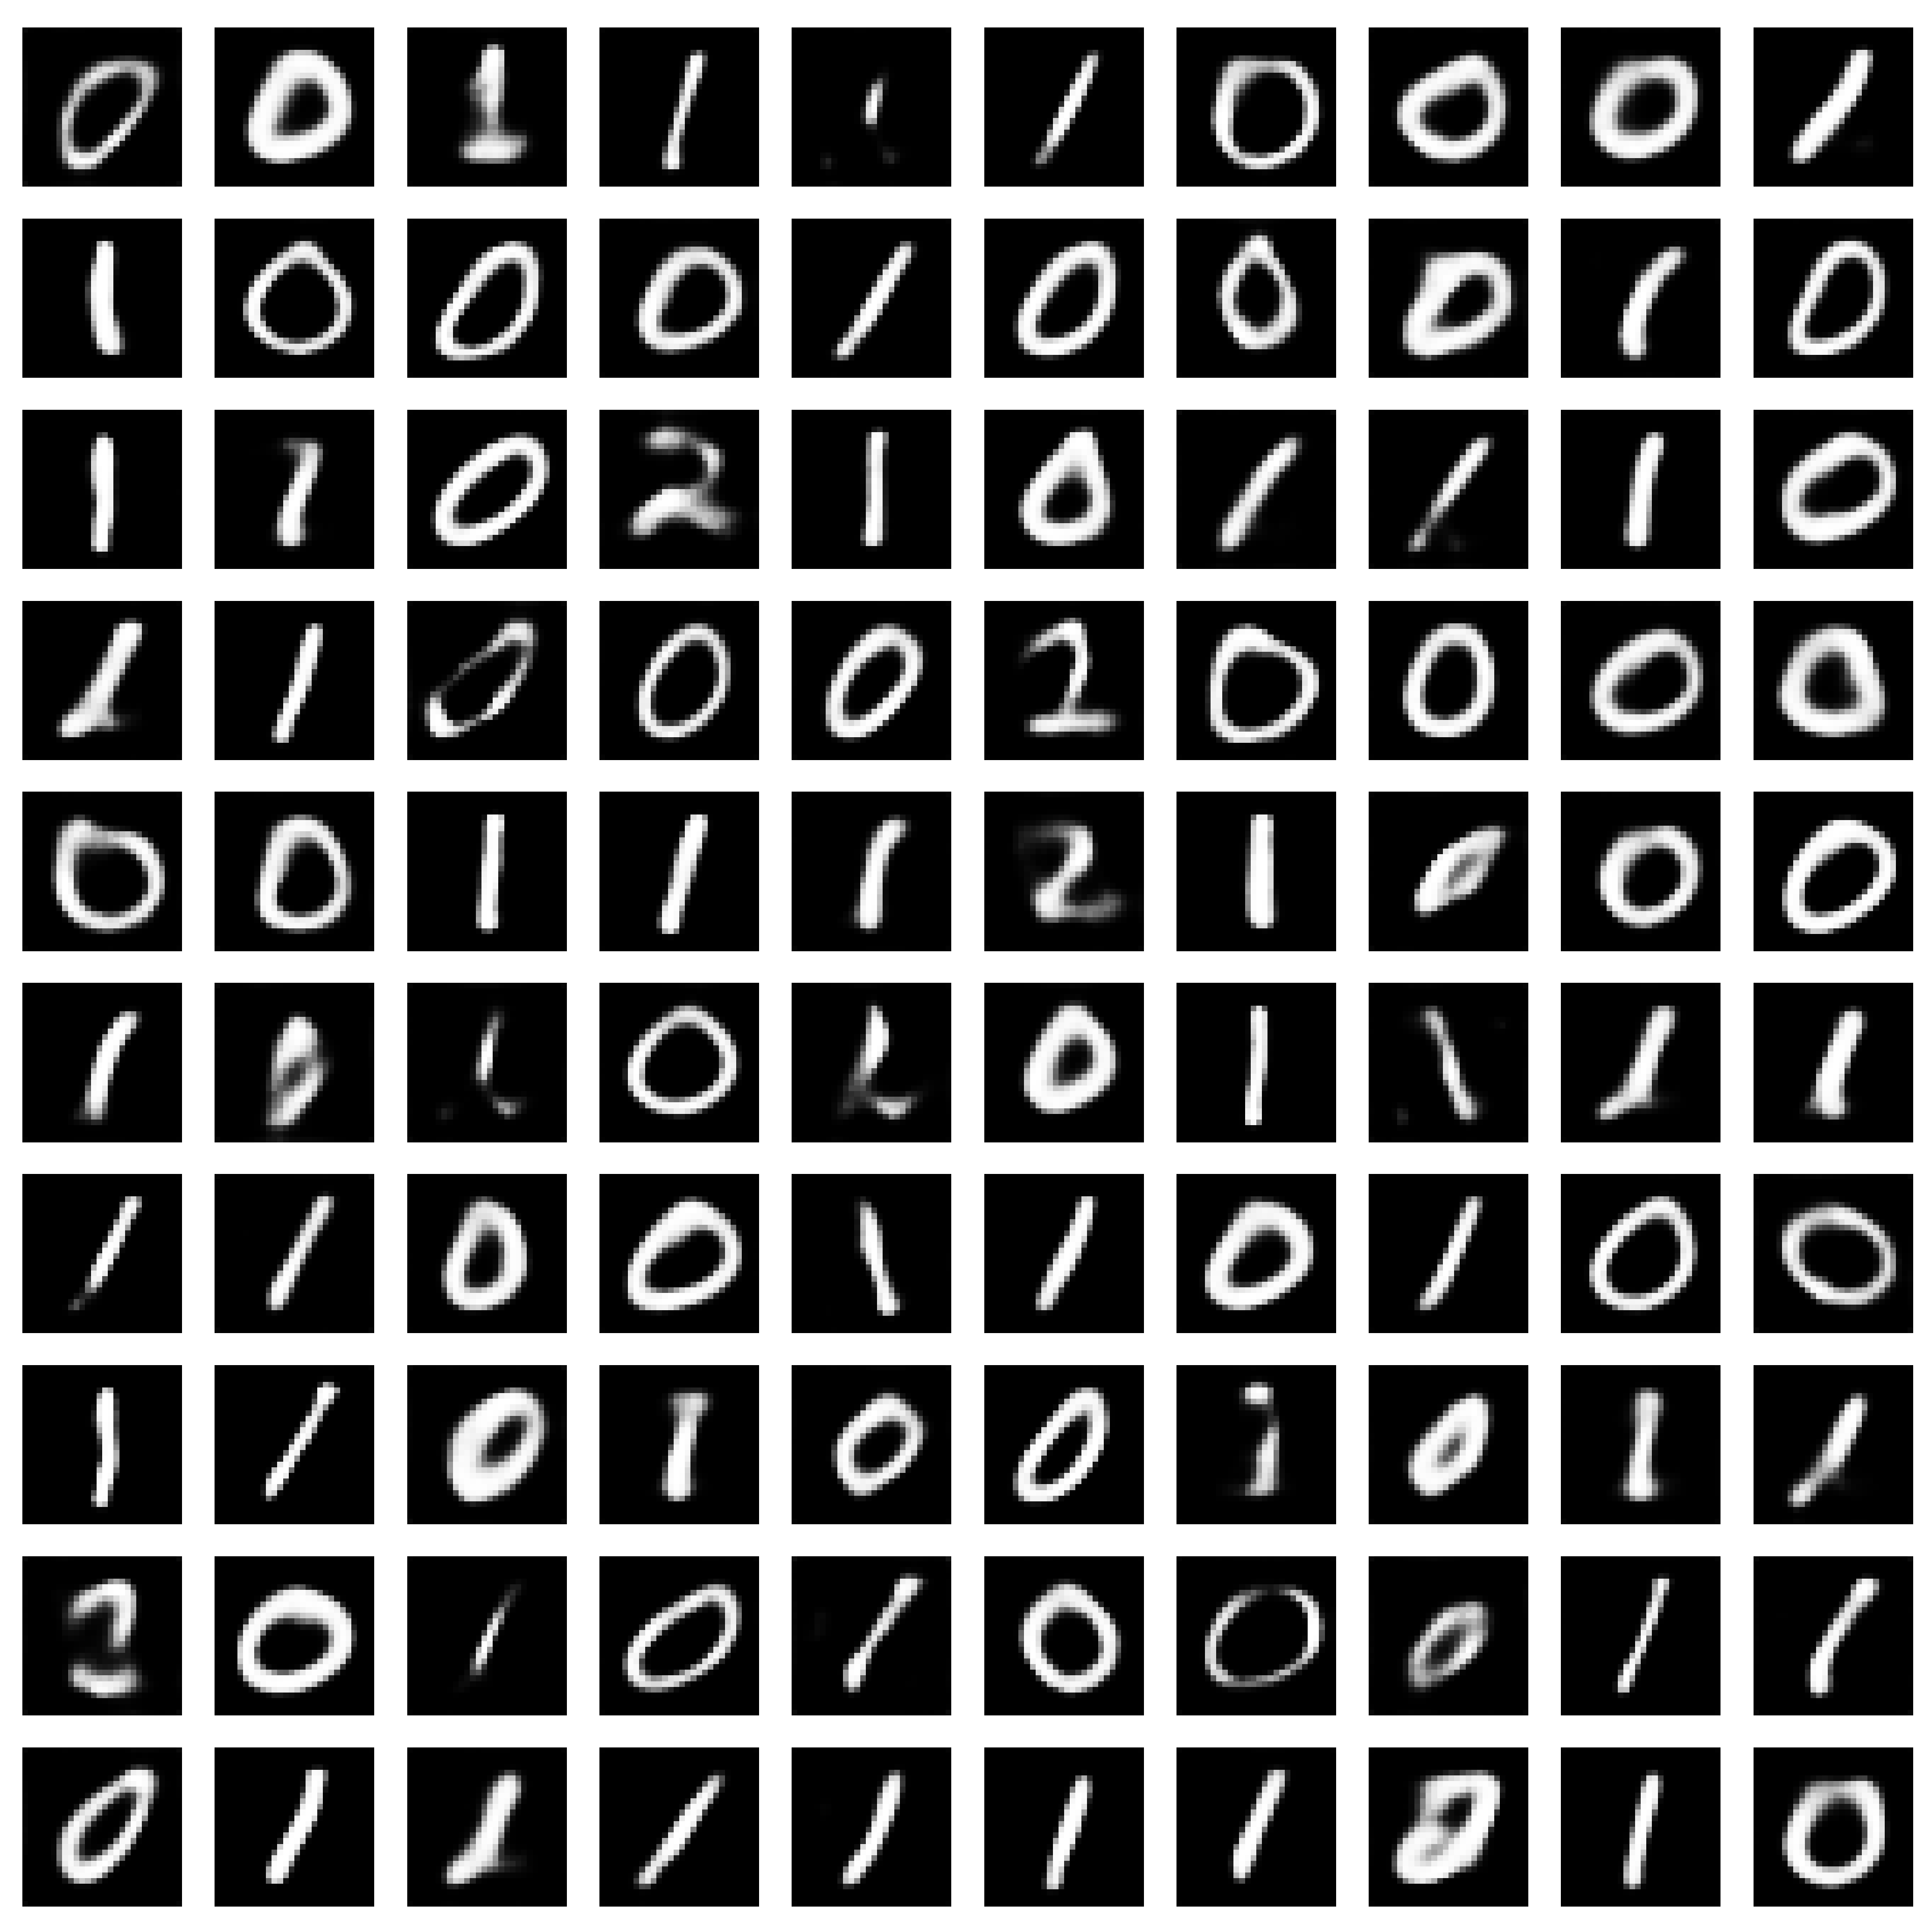
\includegraphics[width=0.8\textwidth]{Figures/PS/ub012_random_generation.png}
%     \end{subfigure}
%     \caption{Random generation of MNIST012: balanced (left) and unbalanced(right)}
%     \label{fig-mnist}
% \end{figure}

\begin{figure}[htb]
    \centering
    \begin{subfigure}{0.24\textwidth}
        \centering
        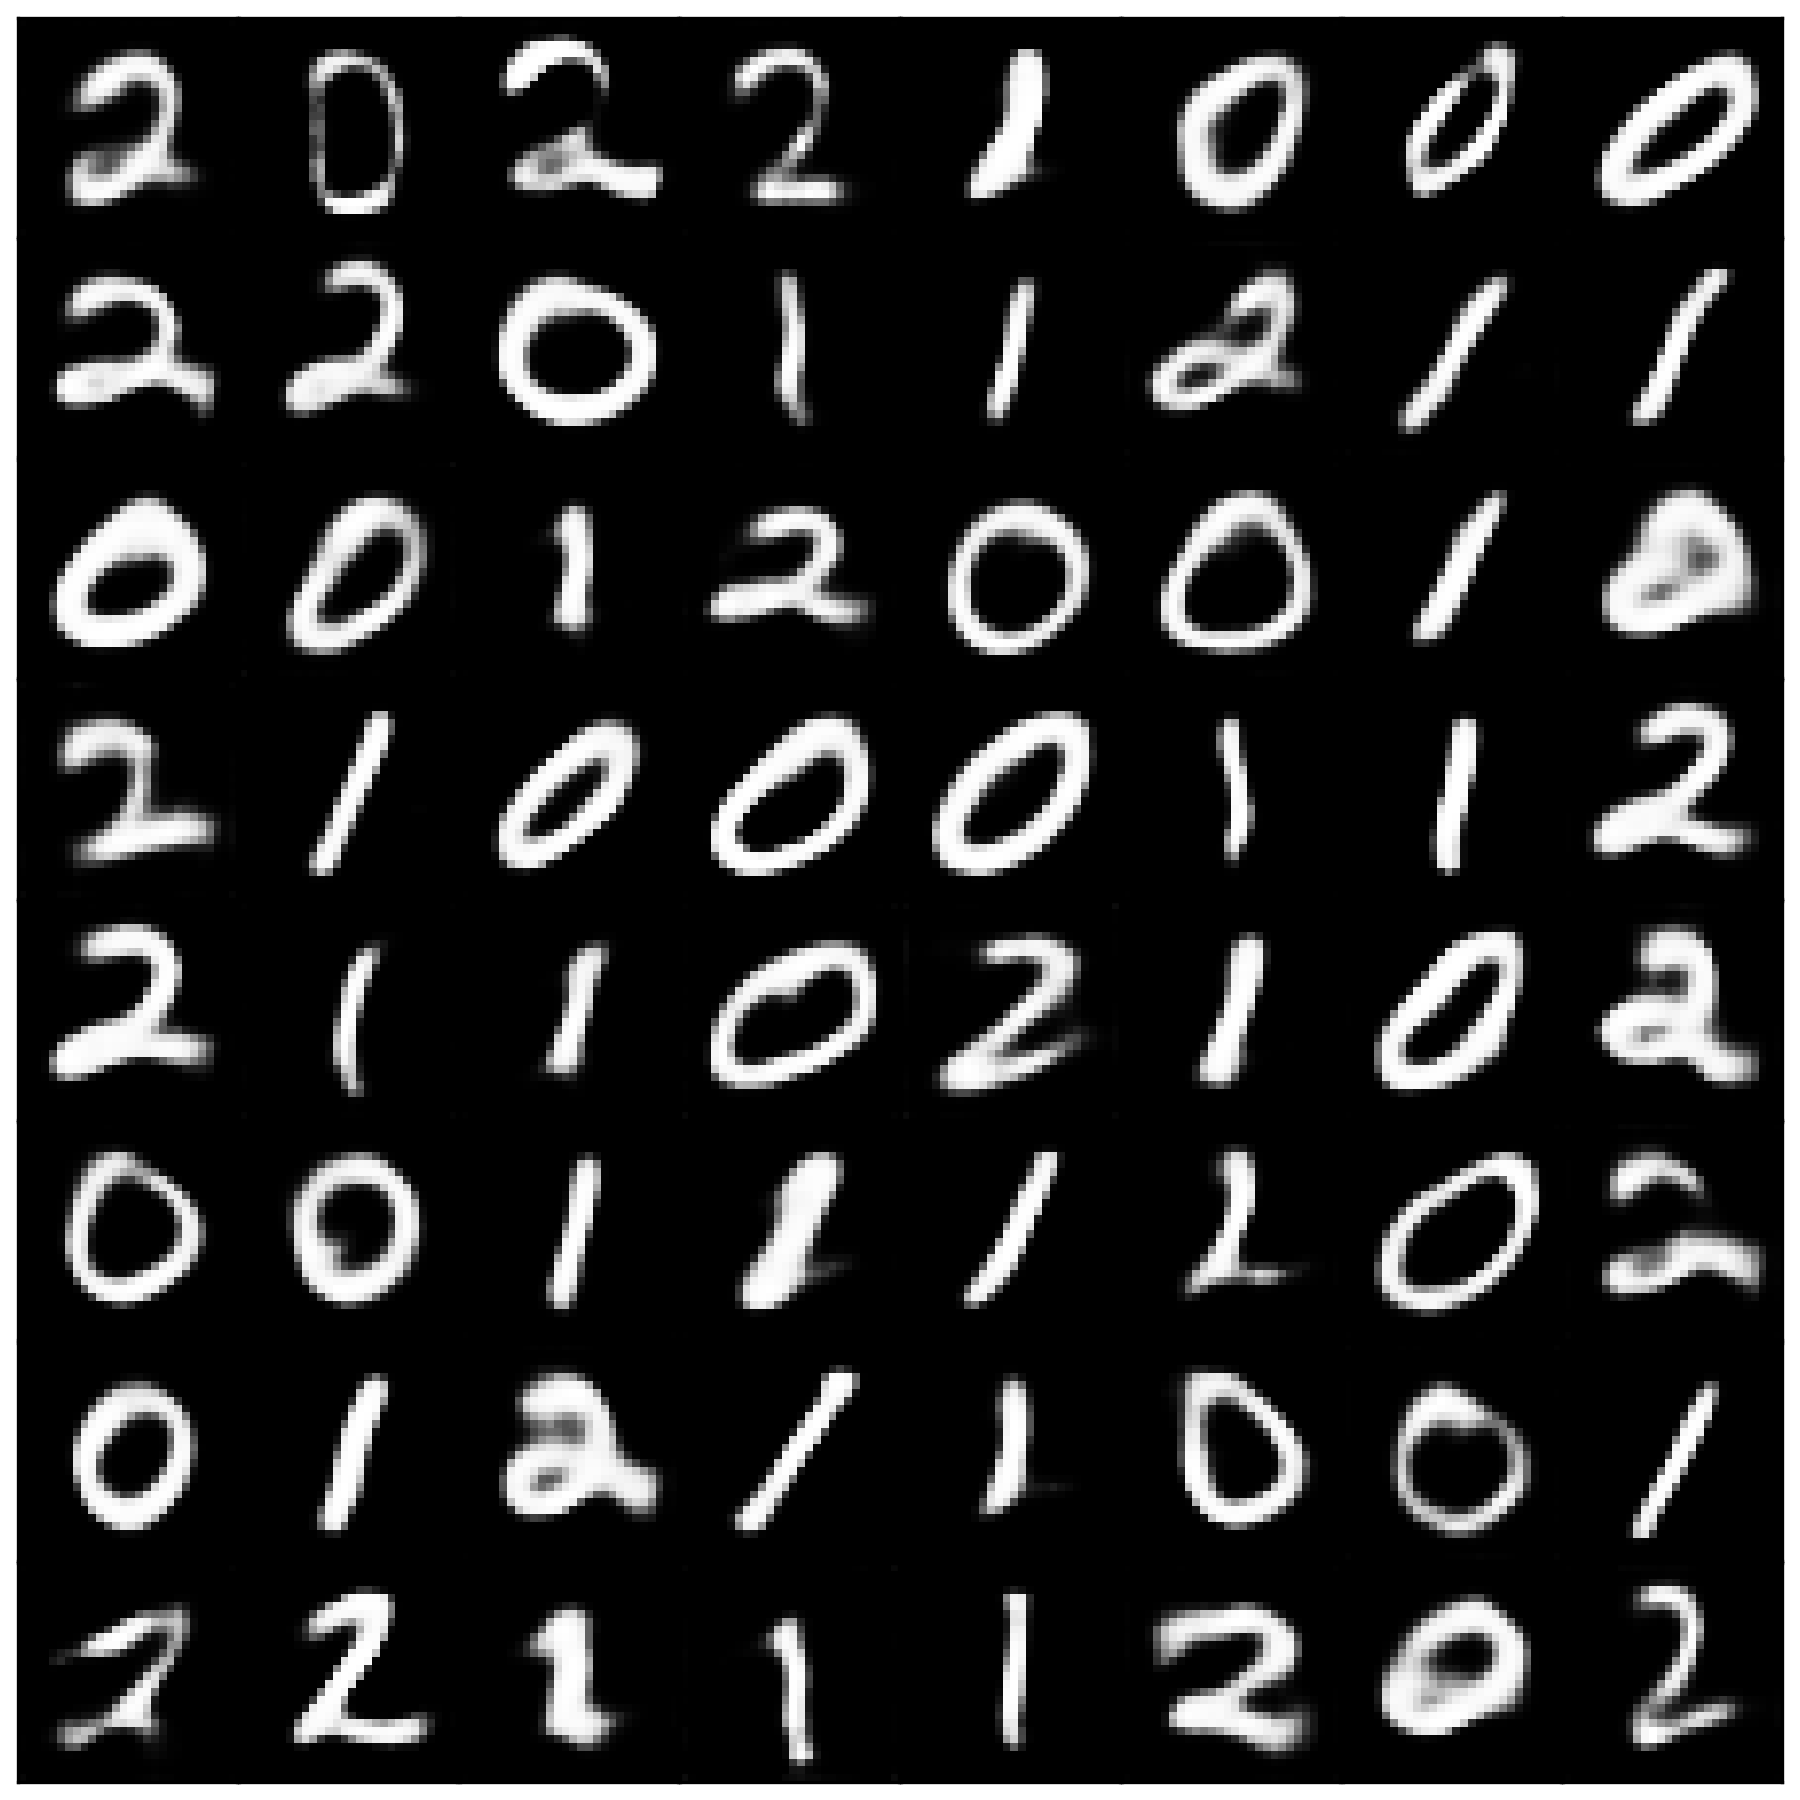
\includegraphics[width=0.9\textwidth]{Figures/PS_v2/genrkm-bMNIST012-gensamples.png}
    \end{subfigure}
    \hfill
    \begin{subfigure}{0.24\textwidth}
        \centering
        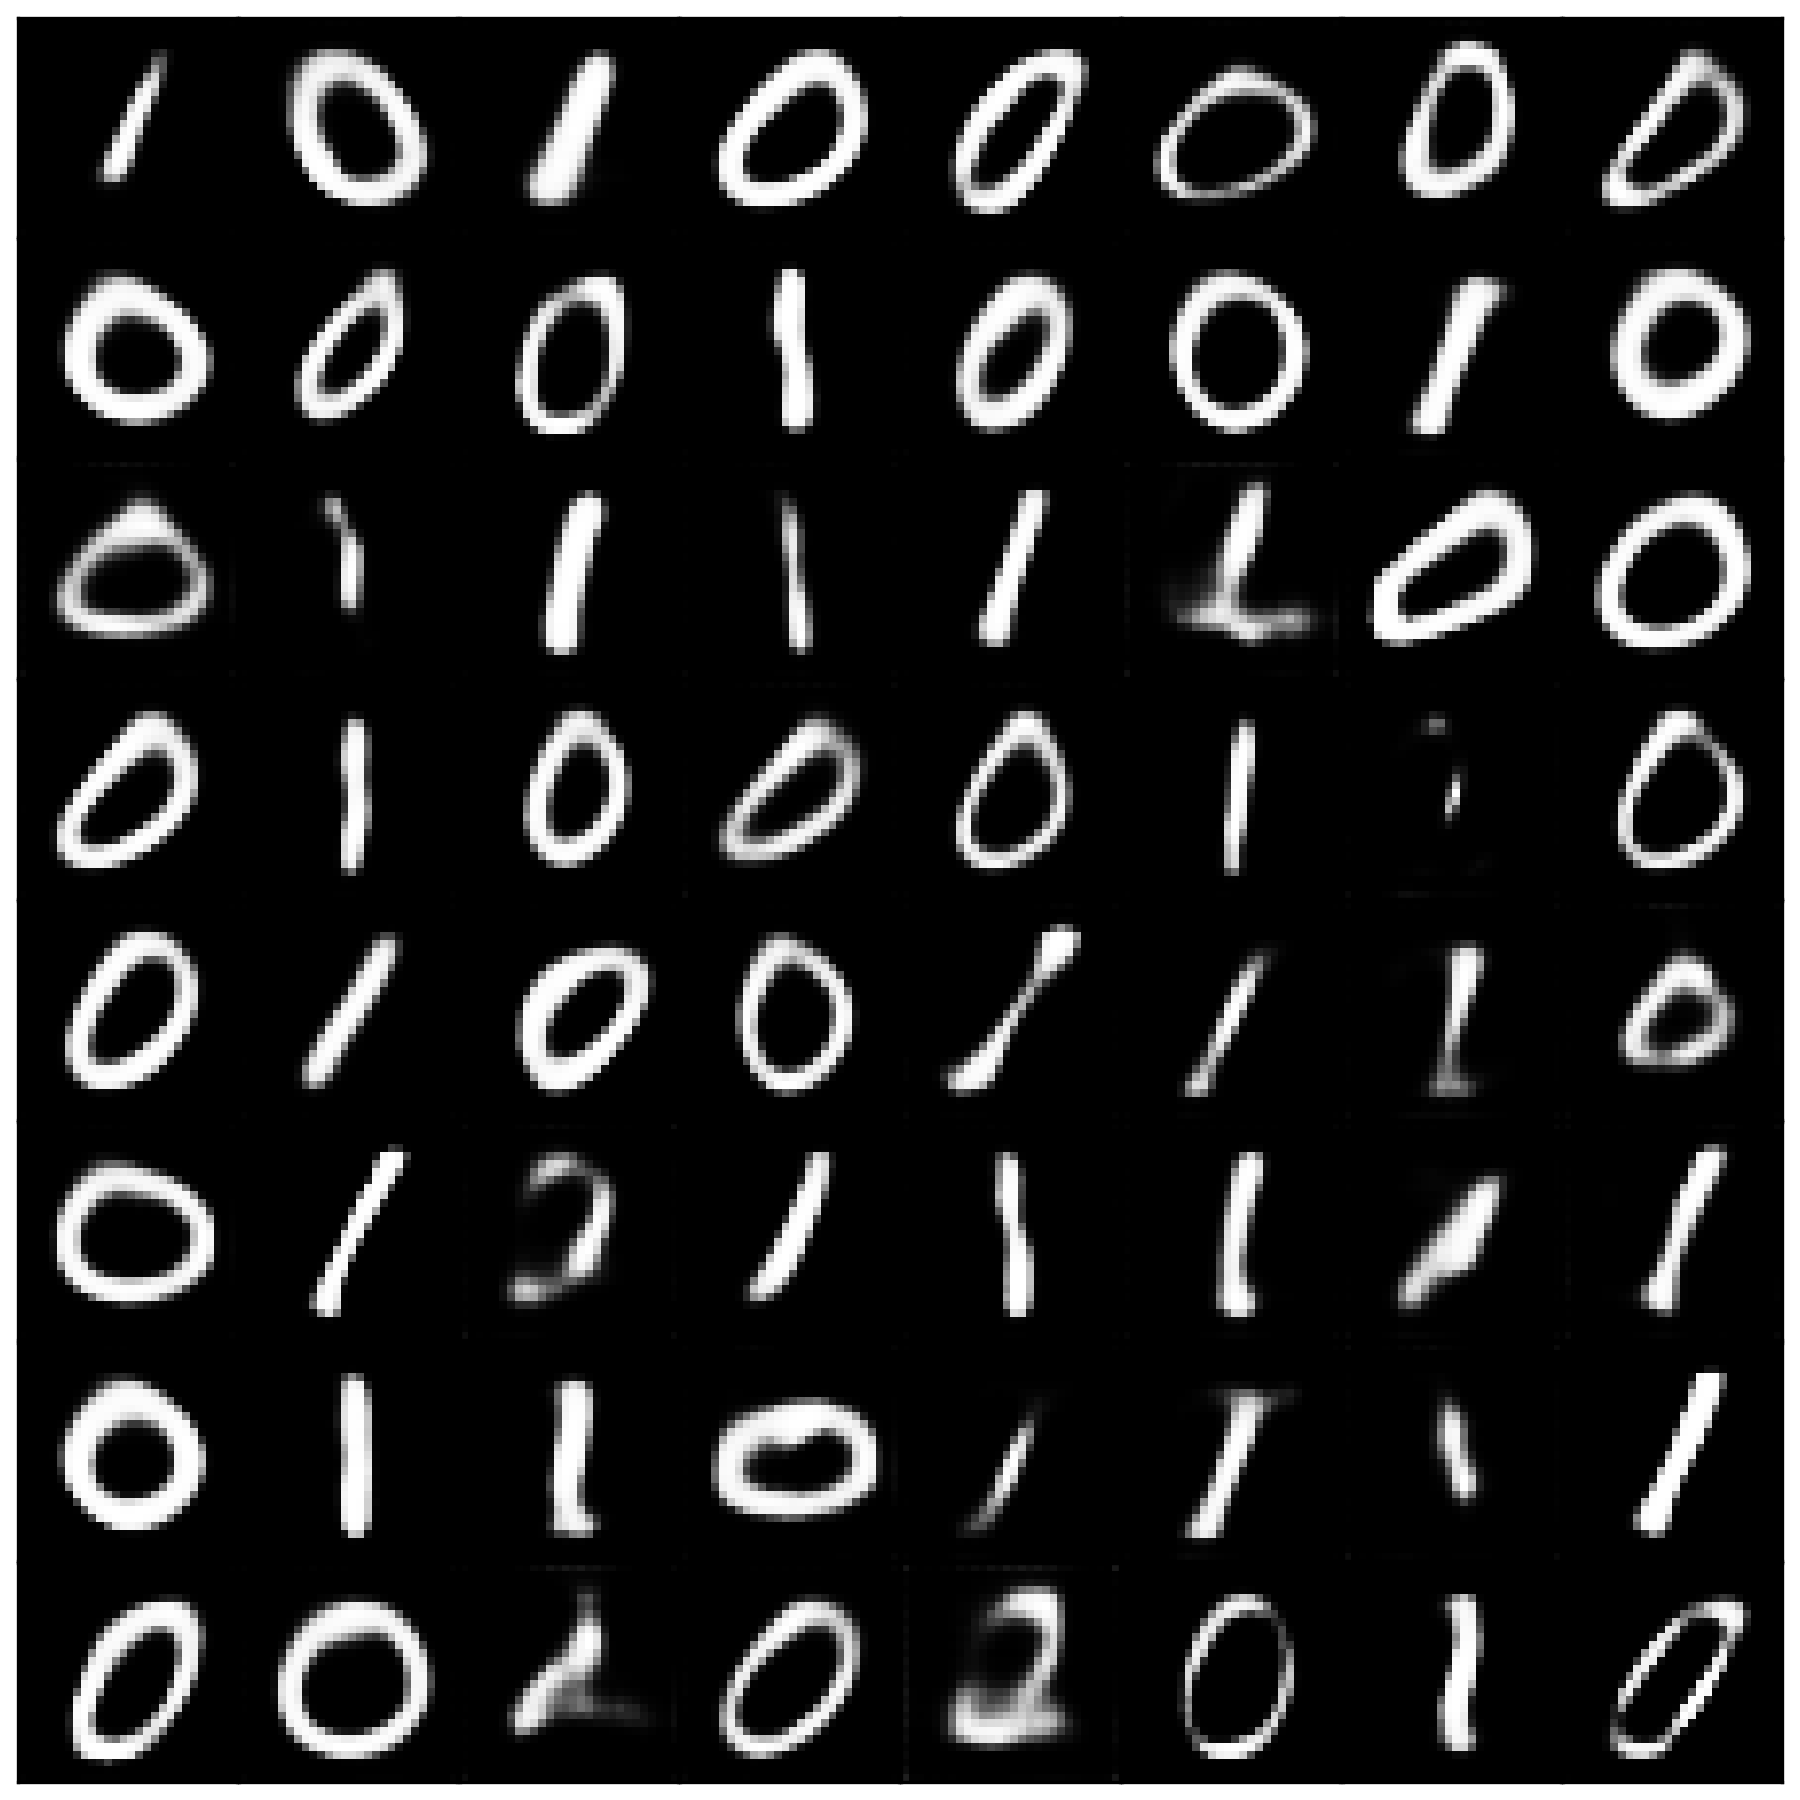
\includegraphics[width=0.9\textwidth]{Figures/PS_v2/genrkm-ubMNIST012-gensamples.png}
    \end{subfigure}
    \hfill
    \begin{subfigure}{0.24\textwidth}
        \centering
        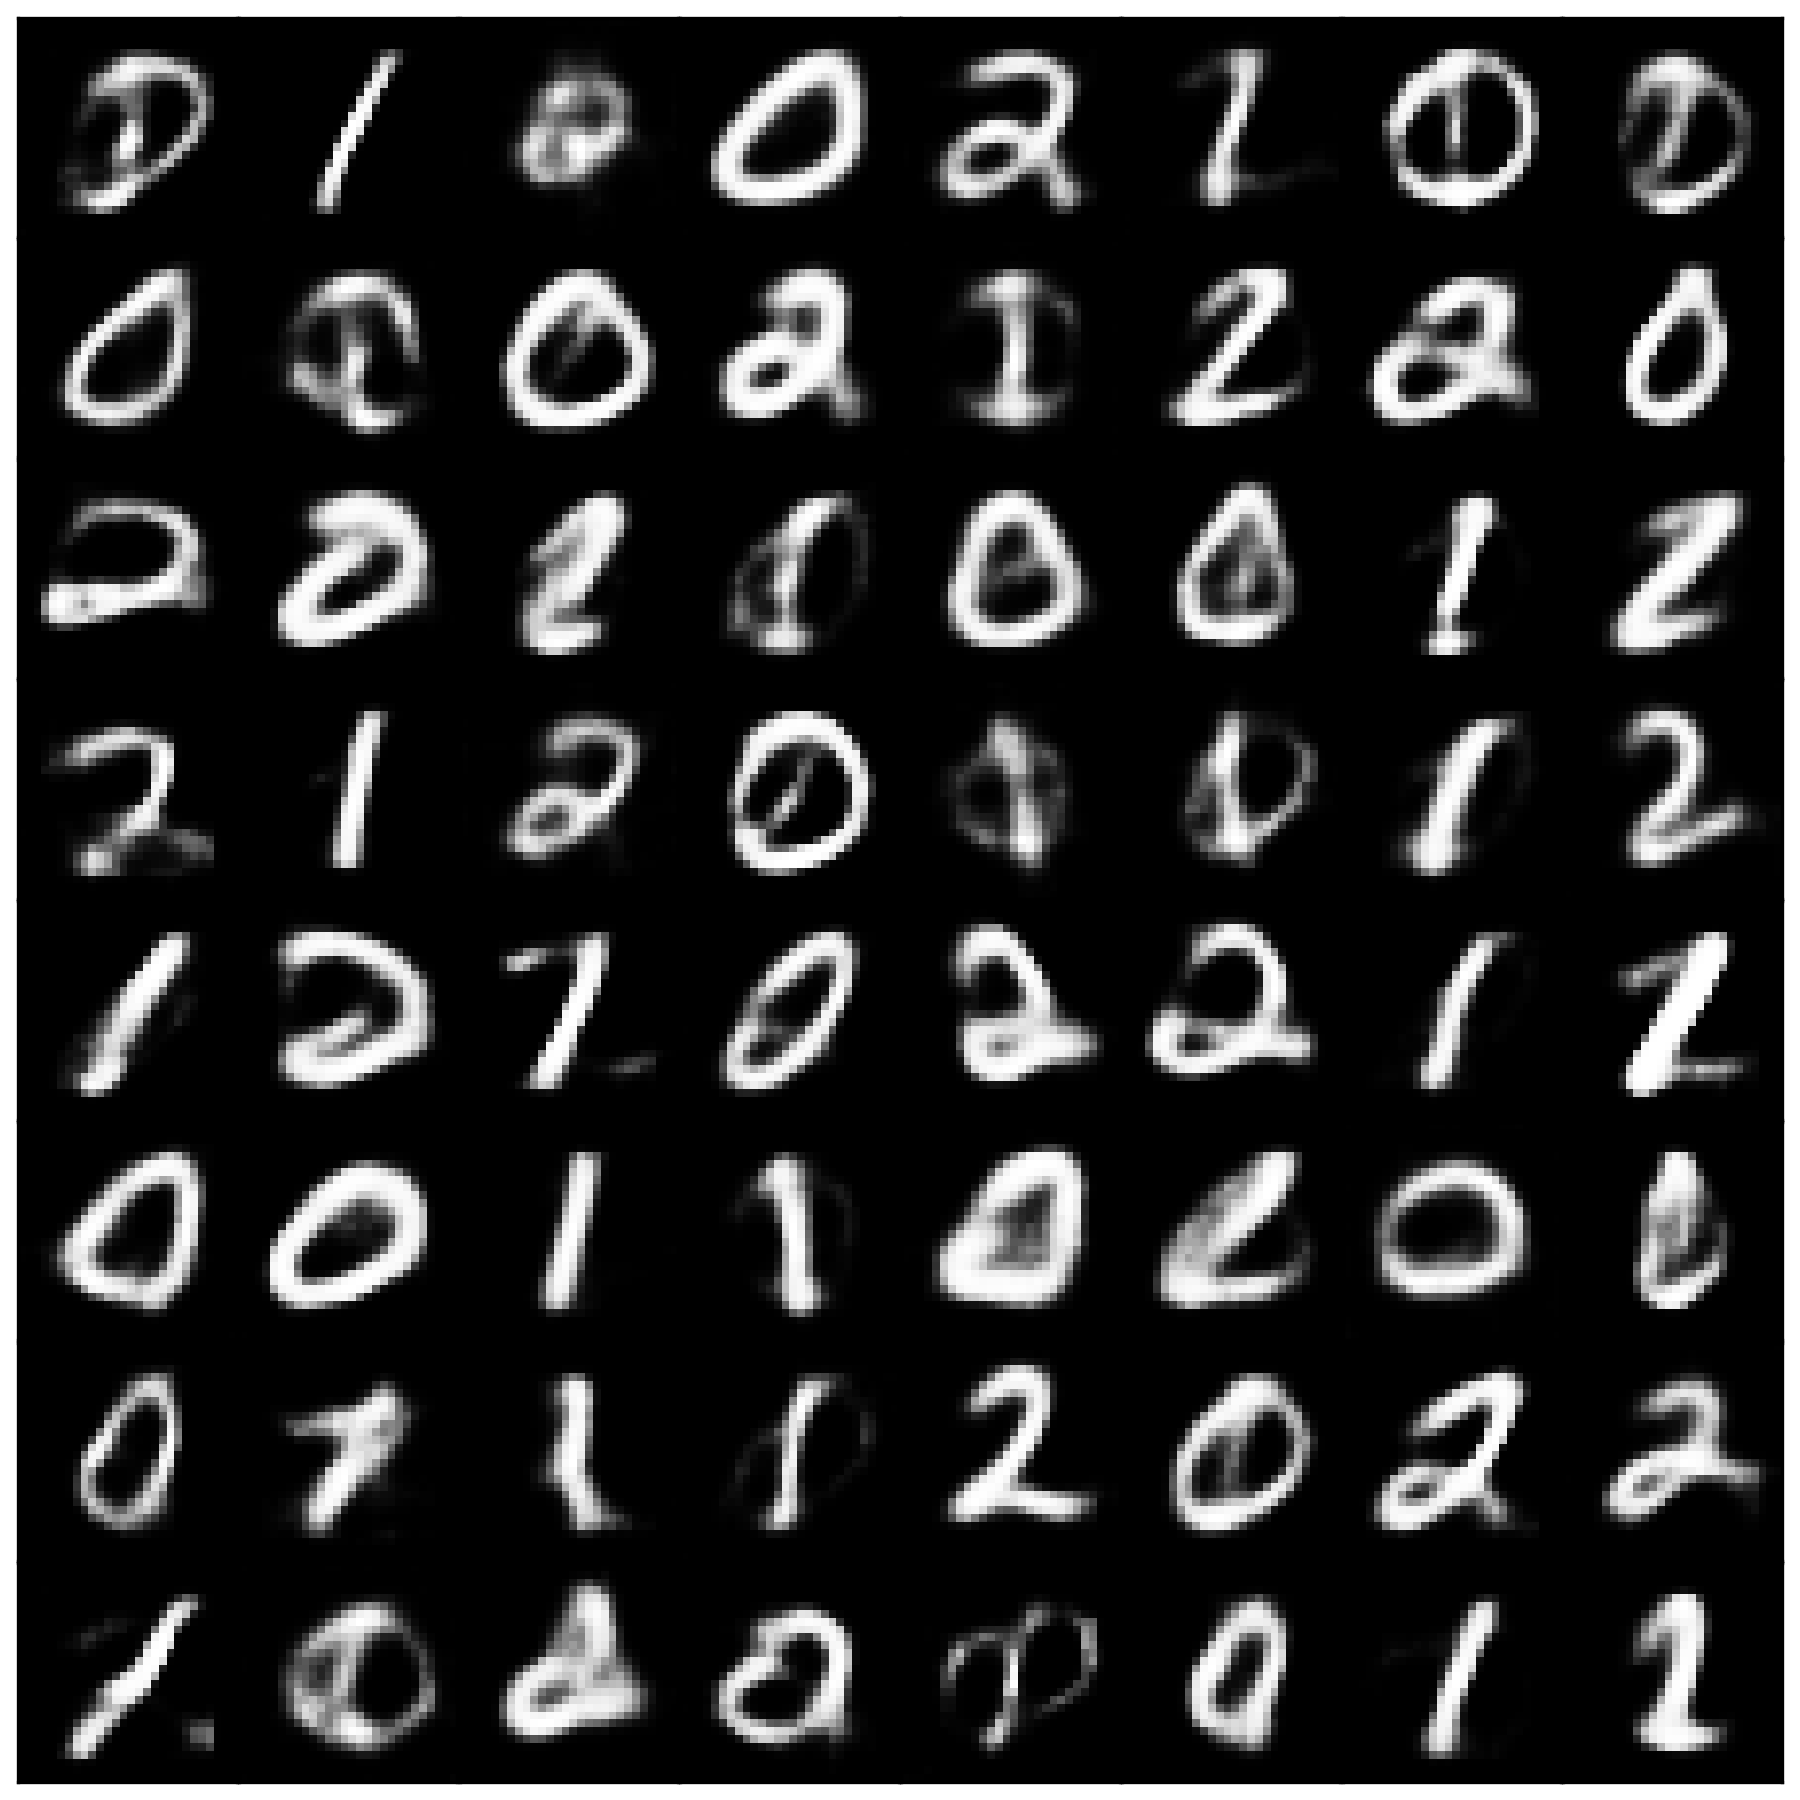
\includegraphics[width=0.9\textwidth]{Figures/PS_v2/vae-bMNIST012-gensamples.png}
    \end{subfigure}
    \hfill
    \begin{subfigure}{0.24\textwidth}
        \centering
        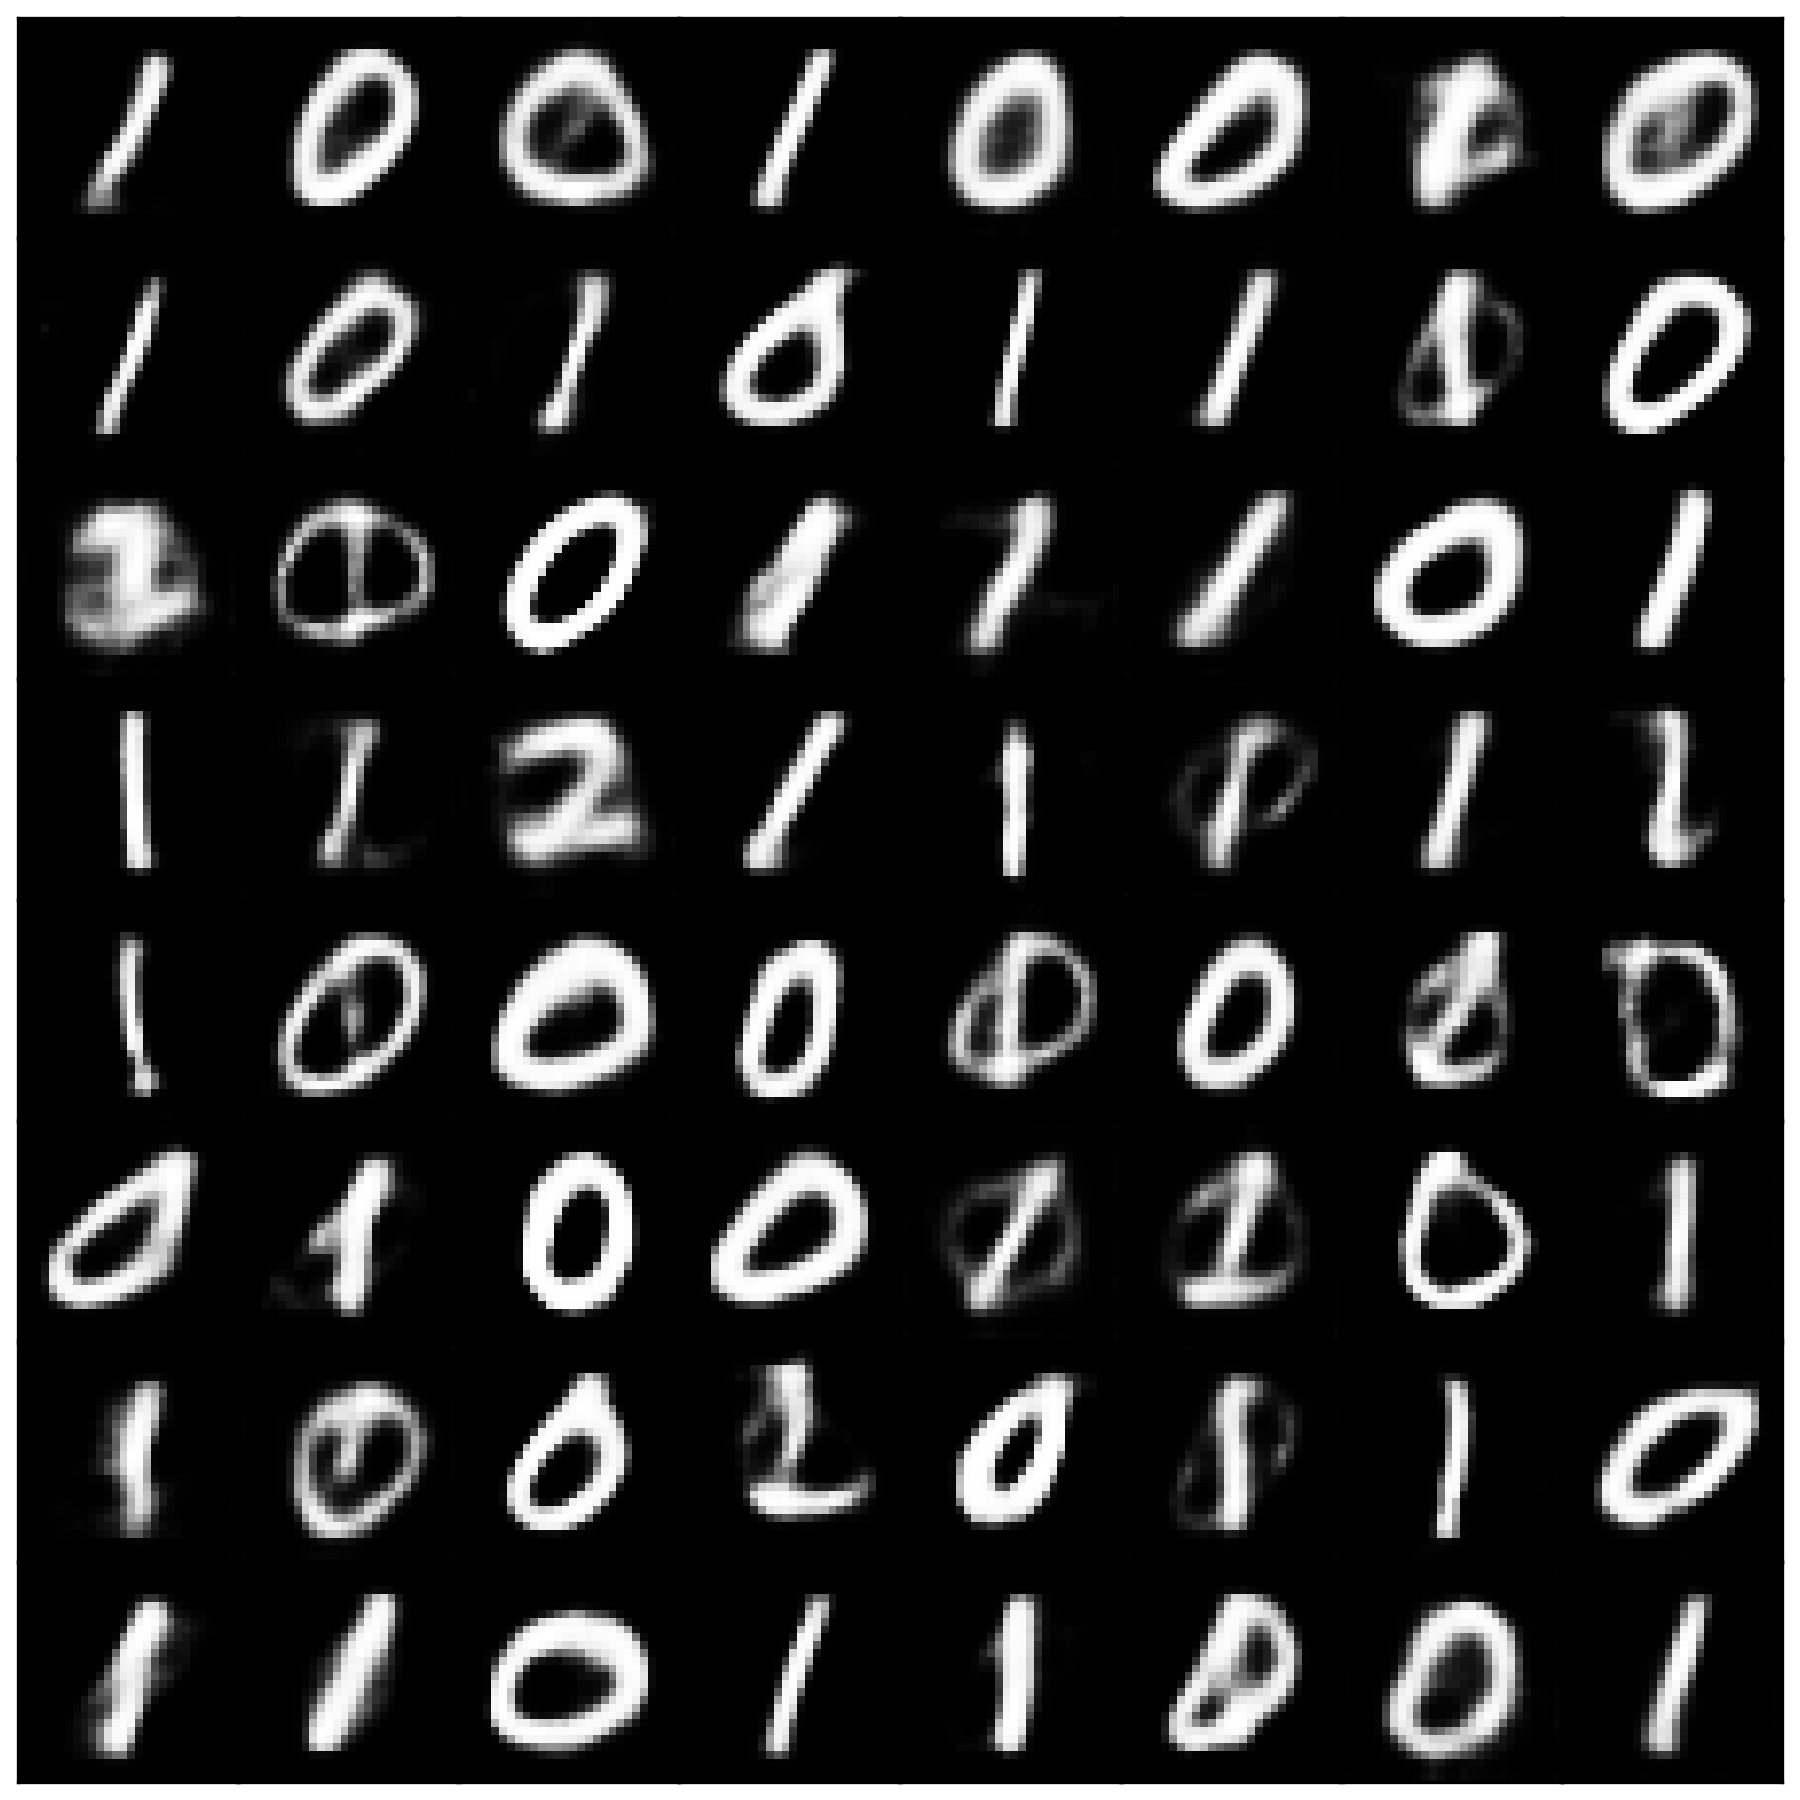
\includegraphics[width=0.9\textwidth]{Figures/PS_v2/vae-ubMNIST012-gensamples.png}
    \end{subfigure}
    \caption{Generated samples from the balanced/unbalanced 012-MNIST dataset by Gen-RKM (first two figures) and VAE (last two figures). The first and the third figures display the generations from a balanced dataset, while the second and the fourth figures show the generations from an unbalanced dataset.}
    \label{fig-mnist}
\end{figure}